\chapter*{CAPÍTULO 3. SocialScrum: Proceso ágil para la gestión de la deuda social}
\addcontentsline{toc}{chapter}{CAPÍTULO 3. SocialScrum: Proceso ágil para la gestión de la deuda social}
\setcounter{chapter}{3}
\setcounter{section}{0}
\setcounter{subsection}{0}
\setcounter{subsubsection}{0}
\renewcommand{\thesection}{\thechapter.\arabic{section}}
\renewcommand{\thesubsection}{\thesection.\arabic{subsection}}
\renewcommand{\thesubsubsection}{\thesubsection.\arabic{subsubsection}}

Este capítulo introduce \gls{socialscrum}, un proceso ágil que nace como una adaptación del marco Scrum, pensado especialmente para abordar la \gls{deuda-social} que suele surgir dentro de los equipos de desarrollo de software.
A lo largo de las siguientes páginas, se exploran las razones que dieron origen a esta propuesta, el modelo conceptual que la respalda, los fundamentos teóricos que la sostienen y, finalmente, el diseño completo del proceso: sus roles, eventos y artefactos.

\section{Introducción}

Aunque Scrum ha demostrado ser una herramienta muy efectiva para gestionar proyectos ágiles, su mirada suele centrarse en lo técnico y deja de lado un aspecto igual de importante: las dinámicas sociales que influyen directamente en la colaboración y el rendimiento del equipo. Con el tiempo, esas tensiones —conocidas como deuda social— pueden acumularse y terminar afectando no solo la calidad del producto, sino también el bienestar y la conexión entre los miembros del equipo \cite{tamburri2013socialdebt}.

De ser pertinente en el análisis, utilizaremos el acrónimo \acrfull{rsl} para referirnos a una Revisión Sistemática de la Literatura.

En respuesta a esta necesidad, surge SocialScrum, un proceso que amplía los principios de Scrum para integrar, de manera explícita, la gestión consciente de la deuda social dentro del propio ciclo ágil.

SocialScrum es un proceso ágil que adapta los principios, eventos y artefactos de Scrum para identificar, priorizar y mitigar la deuda social en equipos de desarrollo de software. Su propósito es hacer visibles las decisiones socio-técnicas subóptimas que impactan la productividad, calidad del software y cohesión del equipo \cite{tamburri2013socialdebt}, integrando prácticas de inspección y adaptación en el plano humano y organizacional \cite{saeeda2024nontechnicaldebt}. En síntesis, promueve un entorno de trabajo saludable y sostenible donde las mejoras sociales y del producto evolucionan de forma armónica. Para ello, SocialScrum introduce roles, eventos y artefactos específicos que complementan los de Scrum, enfocándose en aspectos como la comunicación, colaboración, confianza y bienestar del equipo. A continuación, se presenta un diagrama general del proceso SocialScrum en la figura \ref{fig:socialscrum_overview}.

\begin{figure}[!htbp]
    \centering
    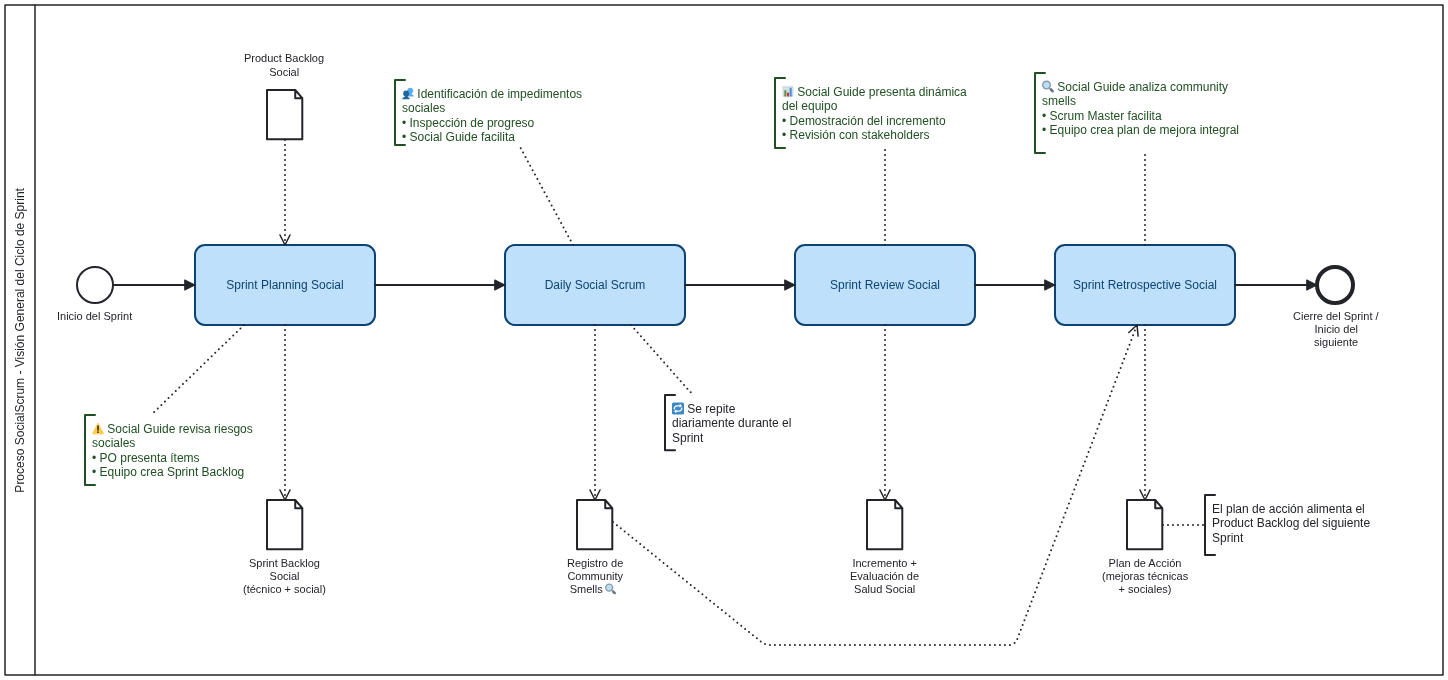
\includegraphics[width=\textwidth]{recursos/socialscrum_vista_general_final.png}
    \caption{Diagrama general del proceso SocialScrum.}
    \label{fig:socialscrum_overview}
\end{figure}

\section{Modelo conceptual de SocialScrum}

Si bien el modelo conserva la estructura fundamental de Scrum, incorpora elementos diseñados específicamente para abordar de frente la deuda social dentro del equipo. Para ello, se basa en los tres pilares empíricos de Scrum: transparencia, inspección y adaptación, aplicándolos directamente al contexto social de los miembros del equipo \cite{schwaber2020scrum}.

A diferencia del Scrum tradicional, que suele centrarse en los aspectos técnicos y del producto, SocialScrum se enfoca en las dinámicas humanas, no solo las visibiliza y las analiza de forma sistemática, sino que también promueve planes de mejora específicos para enfrentar los \glspl{community-smells} y reducir la deuda social \cite{caballero2022communitysmells, tamburri2015insights}.

El modelo SocialScrum se construye sobre tres componentes que se integran al marco Scrum tradicional: roles especializados, eventos adaptados y artefactos enriquecidos con una dimensión social. Estos elementos funcionan de manera coordinada para identificar, analizar y gestionar la deuda social, fortaleciendo tanto el desempeño técnico como el bienestar colectivo del equipo. En conjunto, estas tres dimensiones buscan que las dinámicas humanas reciban la misma atención sistemática que los aspectos técnicos del desarrollo.

\subsection{Roles}

SocialScrum mantiene los tres roles esenciales del marco original: el Product Owner, encargado de maximizar el valor del producto; el Scrum Master, responsable de facilitar el proceso y eliminar impedimentos; y los Developers, quienes transforman los elementos del Product Backlog en incrementos de valor \cite{schwaber2020scrum}.
No obstante, el modelo da un paso más allá al incorporar un cuarto rol especializado, el Social Guide, enfocado en atender la dimensión social del equipo y velar por su equilibrio humano y organizacional.

\subsubsection{Product Owner}

En SocialScrum, el Product Owner conserva su función central de maximizar el valor del producto \cite{schwaber2020scrum}. Sin embargo, recibe del Social Guide información sobre cómo la deuda social puede influir en la predictibilidad y velocidad del equipo. Esa perspectiva le permite tomar decisiones de priorización más conscientes y equilibradas, considerando no solo el valor del producto, sino también la salud del equipo que lo construye.
Su papel en este ámbito se limita a estar informado y valorar las recomendaciones del Social Guide cuando sea pertinente para la planificación del producto, pero sin involucrarse directamente en la gestión o resolución de las dinámicas sociales internas \cite{saeeda2024nontechnicaldebt}.
En otras palabras, el Product Owner se convierte en un aliado informado, no en un actor operativo dentro de la gestión social del equipo.

En SocialScrum, el Product Owner asume tres nuevas responsabilidades que amplían su rol tradicional e incorporan la dimensión social como parte de la gestión del producto:

\begin{enumerate}
    \item Durante el \textit{Sprint Planning}, el Product Owner recibe del Social Guide una evaluación del \textit{Health Score} del equipo, expresada en una escala del 1 al 10. Si este puntaje resulta crítico (por debajo de 4), el Product Owner comprende que el equipo no está en condiciones de asumir \textit{features} de alta complejidad. En ese caso, prioriza en su lugar acciones o elementos orientados a mitigar la deuda social existente.
    \item En cada proceso de priorización, el Product Owner busca equilibrar tres dimensiones: (a) el valor de negocio, (b) la urgencia técnica y (c) la salud social del equipo. Estos factores rara vez se alinean de manera perfecta, por lo que la decisión final requiere diálogo y juicio compartido entre el Product Owner, el Social Guide y el Scrum Master.
    \item El Product Owner no interviene directamente en las dinámicas sociales internas del equipo. Su papel es mantenerse informado y considerar ese contexto al priorizar, reconociendo que un equipo con buena salud social entrega productos de mayor calidad y de forma más sostenible.
\end{enumerate}

La operacionalización detallada de este rol —incluyendo el \textit{framework} de priorización, los protocolos de decisión y ejemplos prácticos— se presenta en el Capítulo 4, Sección 4.4.

\subsubsection{Scrum Master}

El Scrum Master mantiene su papel como facilitador del proceso y protector del equipo frente a interrupciones externas \cite{schwaber2020scrum}. En SocialScrum, trabaja de la mano con el Social Guide para detectar de forma temprana los impedimentos sociales que puedan surgir durante el Sprint. Mientras el Social Guide aporta un enfoque analítico basado en datos —por ejemplo, usando análisis de redes sociales (SNA) o métricas socio-técnicas—, el Scrum Master ofrece una comprensión más vivencial del grupo, ayudando a abrir conversaciones difíciles y facilitar la resolución de conflictos \cite{saeeda2024nontechnicaldebt}. Ambos diseñan estrategias conjuntas que fortalecen la cohesión del equipo, siempre respetando su autoorganización.

Hay que aclarar que el Scrum Master no asume responsabilidades directas en la gestión de la deuda social; esa función recae exclusivamente en el Social Guide. Su rol es más bien de apoyo y colaboración, asegurando que las intervenciones sociales se integren de manera armoniosa dentro del proceso ágil sin generar fricciones ni confusiones en las responsabilidades.

\subsubsection{Developers}

Los Developers conservan su responsabilidad sobre la implementación técnica y la autogestión del trabajo del Sprint \cite{schwaber2020scrum}. Sin embargo, en SocialScrum asumen también un papel activo en el monitoreo de la salud social del equipo, donde deben participar en la detección de community smells durante las ceremonias, proponer acciones de mejora social para el Sprint Backlog y colaborar con el Social Guide brindando retroalimentación sobre la comunicación, la colaboración o la distribución del conocimiento \cite{saeeda2024nontechnicaldebt}. Su participación asegura que las intervenciones sociales sean realistas, aplicables y sostenibles dentro del propio equipo.

\subsubsection{Social Guide}

El Social Guide es la figura central de SocialScrum y su misión es cuidar la dimensión social del equipo. No ocupa un rol jerárquico; más bien, actúa como facilitador y consultor en temas humanos y organizacionales. Su objetivo principal es mantener el equilibrio emocional y relacional del grupo, garantizando que la confianza, la comunicación y la cooperación sean pilares constantes del trabajo.

Sus responsabilidades principales incluyen:

\begin{itemize}
    \item \textbf{Identificación y análisis de \textit{community smells}:} Detecta patrones como el aislamiento, la falta de cooperación o decisiones socio-técnicas poco informadas \cite{saeeda2024nontechnicaldebt}. Para ello, utiliza herramientas como el análisis de redes sociales (SNA) y otras técnicas que ayudan a evaluar la salud de la comunidad de desarrollo.

    \item \textbf{Facilitación de estrategias de mitigación:} Diseña y aplica acciones específicas para atender los problemas detectados, fomentando una comunicación abierta, un entorno de seguridad psicológica y relaciones basadas en el respeto mutuo \cite{saeeda2024nontechnicaldebt, martini2019agiledebt}.

    \item \textbf{Educación y concientización:} Promueve la comprensión colectiva sobre qué es la \textbf{deuda social} y cómo impacta en la productividad y calidad del software \cite{tamburri2015insights}.

    \item \textbf{Colaboración con el Scrum Master:} Trabaja codo a codo con el Scrum Master para identificar y resolver impedimentos sociales, aportando una mirada especializada en la cohesión grupal y la resolución de conflictos \cite{schwaber2020scrum}.

    \item \textbf{Colaboración con el Product Owner:} Informa al Product Owner sobre los efectos de la deuda social en el valor del producto, facilitando una priorización equilibrada entre resultados técnicos y salud del equipo \cite{saeeda2024nontechnicaldebt, tulili2022burnout}.
\end{itemize}

Es fundamental dejar claro lo que el Social Guide \textbf{no hace}:

\begin{itemize}
    \item \textbf{No reemplaza al Scrum Master:} el Scrum Master se encarga de facilitar el proceso ágil; el Social Guide, en cambio, se enfoca en facilitar las dinámicas sociales del equipo. Ambos roles se complementan, no se superponen.
    \item \textbf{No evalúa el desempeño individual:} el Social Guide nunca entrega información personal a recursos humanos ni a la gerencia para fines de evaluación. Los datos que maneja son agregados, confidenciales y usados exclusivamente para la mejora del equipo.
    \item \textbf{No actúa como ``policía social'':} su labor no es sancionar ni imponer normas. Su función es acompañar y guiar al equipo para que identifique y resuelva sus propios conflictos.
    \item \textbf{No toma decisiones sobre el producto:} el Product Owner define qué se construye; el Social Guide simplemente aporta información sobre cuándo el equipo está en condiciones de comprometerse.
\end{itemize}

Para desempeñar el rol de manera efectiva, el Social Guide necesita combinar sensibilidad humana con criterio analítico. Algunas competencias clave son:

\begin{enumerate}
    \item \textbf{Experiencia en dinámicas de grupo:} conocimientos en psicología social (idealmente con especialización en gestión de personas), resolución de conflictos y facilitación de equipos.
    \item \textbf{Comprensión técnica:} conoce el contexto del desarrollo de software —como prácticas de \textit{pair programming}, revisiones de código o despliegues—, aunque no necesariamente sea un programador experto.
    \item \textbf{Capacidad de medición:} sabe interpretar escalas psicométricas, analizar tendencias y traducir datos en acciones comprensibles para el equipo.
    \item \textbf{Neutralidad:} no tiene autoridad ejecutiva; su poder radica en la confianza, la escucha y la capacidad de facilitar sin imponer.
\end{enumerate}

\subsection{Eventos adaptados}

En SocialScrum, los eventos del marco original se ajustan para incorporar la gestión de la deuda social sin modificar su esencia ni su propósito fundamental. Esta adaptación surge de una premisa sencilla pero profunda: si la deuda social es, por naturaleza, algo difícil de ver, que evoluciona con el tiempo y se resiste al cambio —como lo plantean los principios empíricos—, entonces los espacios de inspección y adaptación no pueden quedar sujetos a la casualidad ni a la buena voluntad. Deben estar integrados de manera intencional en la dinámica del equipo, formando parte de su ritmo cotidiano y de su cultura de trabajo.

SocialScrum, por tanto, no añade nuevos eventos; en cambio, aprovecha los mismos espacios del marco Scrum para incluir una dimensión social en ellos.
La clave está en que esta integración se logra sin sacrificar tiempo de desarrollo ni alterar el flujo natural del equipo. Cada evento mantiene su propósito original, pero amplía su alcance para incluir la salud social como un aspecto esencial del desempeño colectivo.

Los ajustes sociales se incorporan respetando el \textbf{Principio de No-Sobrecarga}:

\begin{itemize}
    \item \textbf{Daily Standup:} se añade una pregunta final —``¿Hay algún impedimento social?''— que toma entre 2 y 3 minutos adicionales.
    \item \textbf{Sprint Planning:} se incorpora una breve sección de ``Riesgos Sociales'' (15 minutos) para identificar posibles tensiones o bloqueos humanos que puedan afectar el Sprint. Este tiempo se compensa optimizando otras secciones, sin afectar la calidad de la planificación.
    \item \textbf{Sprint Review:} se reserva un espacio de aproximadamente 10 minutos para presentar el \textit{Health Score} y discutir su evolución durante el Sprint.
    \item \textbf{Sprint Retrospective:} no requiere tiempo adicional; simplemente se reequilibra el enfoque, pasando de una atención predominantemente técnica (90\%) a una distribución más equilibrada entre lo técnico y lo social (50\%-50\%).
\end{itemize}

\textbf{Total:} el tiempo adicional estimado es de aproximadamente 45 minutos por cada Sprint de dos semanas, lo que equivale a unos 4.5 minutos por día.
En términos prácticos, esto representa menos del 1\% del tiempo total del Sprint, una inversión mínima frente al impacto positivo que genera en la salud y sostenibilidad del equipo.

\emph{Referencia:} el Principio de No-Sobrecarga se desarrolla con mayor detalle en el Capítulo 4, Sección 4.3, donde se incluyen tablas de distribución de tiempo por evento y estrategias de optimización para reducir el overhead aún más.

Cada evento incorpora una dimensión social específica, alineada con los valores de Scrum y con los fundamentos teóricos del modelo. La Tabla \ref{tab:eventos_adaptados} muestra cómo cada ceremonia se transforma en un espacio para observar, evaluar y fortalecer la salud social del equipo; un punto de encuentro donde también se inspecciona lo humano, no solo lo técnico.

\begin{adjustwidth}{\parindent}{0pt}
    \begin{table}[!htbp]
        \caption{Eventos de Scrum adaptados en SocialScrum}
        \label{tab:eventos_adaptados}
        \centering
        \renewcommand{\arraystretch}{1.2}
        \small
        \begin{tabularx}{\dimexpr\textwidth-\parindent\relax}{@{}p{3.2cm}X@{}}
            \toprule
            \textbf{Evento}               & \textbf{Adaptación en SocialScrum}                                                                                                                                                                                     \\
            \midrule

            \textbf{Sprint Planning}      &
            Se incorpora una \textbf{Revisión de Riesgos Sociales}, liderada por el Social Guide. En esta etapa, el equipo analiza si su estado social actual —medido mediante el \textit{Health Score} y los \textit{smells} activos— le permite comprometerse con tareas de alta complejidad. Se identifican posibles obstáculos sociales y se definen acciones preventivas que se integran directamente en el \textit{Sprint Backlog Social} \cite{schwaber2020scrum}.
            Esta práctica fortalece la \textbf{autonomía} del equipo al permitirle reconocer su capacidad real, y promueve la \textbf{integridad} al hacer visibles sus compromisos sociales.                                                                      \\[1pt]

            \textbf{Daily Standup}        &
            Se añade una pregunta breve pero significativa: ``¿Hay algún impedimento social?''.
            El Social Guide observa las dinámicas del equipo —quién participa, quién se mantiene en silencio, el tono emocional del grupo— como señales tempranas de posibles tensiones. Si surgen fricciones, se documentan para abordarlas fuera del Daily, respetando el \textit{time-boxing} \cite{saeeda2024nontechnicaldebt}.
            Este enfoque normaliza la conversación sobre dificultades interpersonales y fomenta una transparencia constante en las relaciones del equipo.                                                                                                          \\[1pt]

            \textbf{Sprint Review}        &
            Además de presentar el Increment, se dedican entre 5 y 7 minutos a una \textbf{Evaluación de la Dinámica del Equipo}.
            El Social Guide comparte de forma breve la evolución de las métricas sociales —como SNA o distribución de conocimiento—, los \textit{smells} mitigados o nuevos, y cómo las interacciones influyeron en la entrega.
            Este espacio permite que los stakeholders comprendan que la salud social también incide en el valor del producto \cite{schwaber2020scrum}, visibilizando un aspecto a menudo ignorado y mostrando una preocupación genuina por el bienestar colectivo. \\[1pt]

            \textbf{Sprint Retrospective} &
            Se convierte en el núcleo de la gestión social. El Social Guide lidera una sección específica (de 20 a 30 minutos) estructurada en cuatro fases: revisión del registro de \textit{smells}, análisis de causas raíz (por ejemplo, con la técnica de los ``5 Whys''), diseño de experimentos de mejora con hipótesis comprobables y priorización de las acciones resultantes para el siguiente Sprint.
            Las mejoras sociales más importantes se formalizan con responsables, métricas de éxito y criterios de evaluación \cite{martini2019agiledebt}.
            Este evento encarna el ciclo completo de inspección, adaptación y nueva transparencia, y requiere tanto coraje para abordar los temas difíciles como compromiso para sostener los cambios en el tiempo.                                                \\
            \bottomrule
        \end{tabularx}
    \end{table}
\end{adjustwidth}

Al incorporar nuevas dimensiones sociales dentro de los eventos existentes, SocialScrum busca que la gestión de la deuda social no se perciba como una tarea adicional o un ``pendiente'' más en la agenda del equipo, sino como una parte natural de su dinámica ágil. El objetivo es que estos espacios sociales se integren orgánicamente en el flujo de trabajo, promoviendo una cultura donde lo humano y lo técnico convivan en equilibrio. Así, se fortalece tanto la calidad del producto como las relaciones que lo hacen posible.

La Tabla \ref{tab:eventos-tiempo} presenta una estimación del tiempo adicional (\textit{overhead}) que implican estas adaptaciones, evidenciando que el impacto temporal es mínimo en comparación con los beneficios obtenidos en cohesión, confianza y sostenibilidad del equipo.

\begin{table}[h]
    \centering
    \small
    \begin{tabular}{|l|c|c|c|}
        \hline
        \textbf{Evento}      & \textbf{Tiempo estimado} & \textbf{Overhead social} & \textbf{Facilitador}                                \\
        \hline
        Daily Standup        & 15 min                   & +2-–3 min                & Social Guide (1 pregunta)                           \\
        Sprint Planning      & 4 h                      & +15 min                  & Social Guide (revisión de riesgos sociales)         \\
        Sprint Review        & 2 h                      & +10 min                  & Social Guide (evaluación del \textit{Health Score}) \\
        Sprint Retrospective & 1.5 h                    & +0 min                   & Scrum Master (técnico) + Social Guide (social)      \\
        \hline
    \end{tabular}
    \caption{Overhead temporal de los eventos sociales en SocialScrum}
    \label{tab:eventos-tiempo}
\end{table}

\emph{Nota: El principio de \textbf{No Sobrecarga} establece que estas adaptaciones deben integrarse en los eventos existentes de Scrum sin aumentar de forma significativa el tiempo total de las ceremonias. Este principio se desarrolla con mayor detalle en el Capítulo 4, Sección 4.3.}

\FloatBarrier

El \textbf{Sprint Retrospective Social} es, sin duda, el evento que mayor protagonismo tiene dentro del ciclo de gestión social, ya que marca el cierre natural del proceso y el punto de partida para nuevas mejoras. A diferencia de las retrospectivas tradicionales —donde los temas humanos suelen abordarse solo de manera tangencial—, aquí se convierten en el eje central de la conversación, con una estructura clara, propósito definido y un enfoque deliberado en el bienestar colectivo.

La Figura \ref{fig:sprint_retrospective_social1} ilustra el flujo completo. El proceso comienza con la presentación del Social Guide, quien comparte tanto datos cuantitativos —como métricas del Sprint y tendencias del \textit{Health Score}— como observaciones cualitativas sobre las interacciones del equipo. A partir de esta base, el grupo analiza de forma colaborativa las causas de los \textit{smells} identificados, evitando soluciones rápidas o paliativas.
Las acciones resultantes se formulan como experimentos con hipótesis claras, métricas de éxito y criterios definidos para decidir si continuar, ajustar o descartar el cambio. Esta lógica experimental refleja el espíritu empírico y de aprendizaje continuo que caracteriza a SocialScrum.

En este flujo, todos los roles tienen un papel activo y complementario. El Social Guide aporta el diagnóstico analítico y orienta la conversación hacia los aspectos relacionales; el Scrum Master facilita los diálogos difíciles y protege el ambiente psicológico del grupo; los Developers proponen soluciones prácticas y contextualizadas; y el Product Owner actualiza el \textit{Product Backlog Social} con las acciones resultantes.
De esta manera, la gestión social deja de ser responsabilidad de una sola figura y se convierte en un compromiso compartido que refuerza la madurez y cohesión del equipo.

\textbf{Criterios de éxito:}
\begin{itemize}
    \item Se analizó en profundidad al menos un \textit{smell} crítico, abordando sus causas reales y no solo sus síntomas.
    \item Las acciones acordadas se formularon como hipótesis comprobables, con métricas claras que permitan evaluar su efectividad.
    \item El equipo pudo expresar sus inquietudes con libertad y sin temor a represalias, reflejando un entorno de auténtica seguridad psicológica.
    \item Se identificaron aprendizajes concretos del Sprint anterior, tanto sobre lo que funcionó como sobre aquello que requiere ajuste o mejora.
\end{itemize}

\begin{figure}[!htbp]
    \centering
    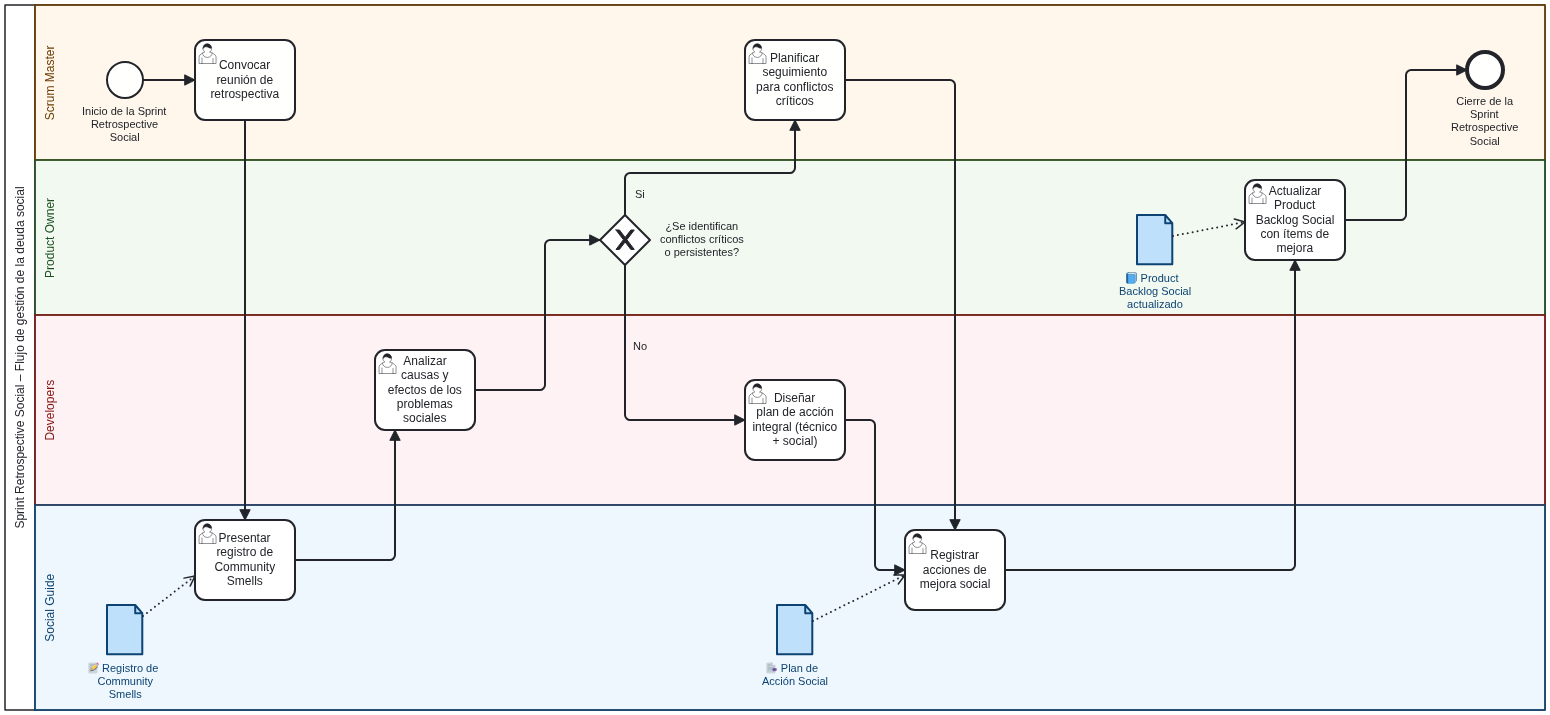
\includegraphics[width=\textwidth]{recursos/sprint-retrospective.png}
    \caption{Flujo detallado del evento Sprint Retrospective Social en el modelo SocialScrum.}
    \label{fig:sprint_retrospective_social1}
\end{figure}

La descripción completa del proceso —con facilitadores, tiempos sugeridos, preguntas guía y herramientas de apoyo— se desarrolla en el Capítulo 4, Sección 4.4, donde se presenta el manual práctico de implementación del modelo.

\FloatBarrier

\subsection{Artefactos sociales}

En Scrum, los artefactos —Product Backlog, Sprint Backlog e Increment— representan el trabajo y el valor generados, y están diseñados para mantener la transparencia en todo momento \cite{schwaber2020scrum}. En SocialScrum, estos artefactos se amplían para incluir la dimensión social, no como un añadido superficial, sino como una extensión natural del principio de transparencia aplicado a los aspectos humanos del equipo.

Si la deuda social influye directamente en el valor del producto —porque retrasa entregas, degrada la calidad o genera retrabajo—, entonces debe abordarse con el mismo nivel de rigor que la deuda técnica. Los artefactos adaptados en SocialScrum buscan justamente eso: transformar los problemas sociales en elementos visibles, medibles y gestionables, con el mismo nivel de importancia que cualquier funcionalidad técnica.

La Tabla \ref{tab:artefactos_adaptados} ilustra cómo cada artefacto se enriquece con información social, manteniendo su propósito original, pero ampliando su alcance hacia la sostenibilidad del equipo y la salud del entorno de trabajo.

\begin{adjustwidth}{\parindent}{0pt}
    \begin{table}[!htbp]
        \caption{Artefactos de Scrum adaptados en SocialScrum}
        \label{tab:artefactos_adaptados}
        \centering
        \renewcommand{\arraystretch}{1.15}
        \small
        \begin{tabularx}{\dimexpr\textwidth-\parindent\relax}{@{}p{2.8cm}X@{}}
            \toprule
            \textbf{Artefacto}       & \textbf{Adaptación en SocialScrum}                                                                                                                                                                                                 \\
            \midrule

            \textbf{Product Backlog} &
            Se amplía con \textbf{Elementos de Deuda Social} o \textbf{Habilitadores de Salud del Equipo}: iniciativas destinadas a mejorar la comunicación, reducir \textit{smells} persistentes o fortalecer las habilidades sociales del grupo (por ejemplo: ``Establecer protocolos de \textit{code review} no tóxicos para mitigar \textit{Priggish Members}'').
            El Product Owner los prioriza junto al Social Guide considerando cuatro criterios: el \textit{Health Score} actual del equipo, la severidad del smell, el impacto en la velocidad y la viabilidad de mitigación \cite{saeeda2024nontechnicaldebt}.
            Este enfoque reconoce que cuidar la salud social también es entregar valor, no una distracción. Refuerza la capacidad del equipo para gestionar su propia complejidad (habilidad) y fomenta la mejora continua mediante herramientas concretas (competencia). \\[1pt]

            \textbf{Sprint Backlog}  &
            Integra explícitamente las \textbf{Acciones de Mitigación Social} como ítems formales, con descripción clara, responsables asignados, esfuerzo estimado y criterios de aceptación definidos.
            Ejemplo: ``Implementar sesiones semanales de ‘lunch \& learn’ sobre el subsistema X.
            Owner: Developer A + voluntario rotativo.
            DoD: Al menos tres desarrolladores pueden explicar la arquitectura básica.
            Métrica: reducción superior al 30\% en preguntas a Developer A (medido en Slack).''
            Esta visibilidad asegura que el trabajo social no sea ``invisible'', sino parte integral del compromiso del Sprint \cite{saeeda2024nontechnicaldebt}.
            Formaliza la responsabilidad colectiva (compromiso) y potencia la \textbf{autonomía} del equipo para definir cómo abordar sus propios retos interpersonales.                                                                                                  \\[1pt]

            \textbf{Incremento}      &
            Además de cumplir con la \textit{Definition of Done} técnica, cada Incremento se evalúa también por su \textbf{Impacto en la Salud Social}.
            El Social Guide participa en la definición de criterios de sostenibilidad social, respondiendo preguntas como: ¿el trabajo se completó sin generar burnout? ¿sin crear nuevos \textit{smells} (por ejemplo, \textit{Black Clouds} por falta de documentación)? ¿mejoraron las dinámicas de colaboración?
            Se analizan indicadores como variaciones en el \textit{Health Score}, aparición o reducción de \textit{smells}, distribución del conocimiento (SNA) o niveles de carga emocional (horas extra, rotación).
            Un Incremento que cumple lo técnico pero deteriora el bienestar del equipo debe considerarse deuda social acumulada \cite{saeeda2024nontechnicaldebt}.
            Este equilibrio entre entrega técnica y sostenibilidad humana fortalece el valor de \textbf{foco} y refleja la \textbf{relacionalidad} del equipo al medir su cohesión y colaboración efectiva.                                                               \\
            \bottomrule
        \end{tabularx}
    \end{table}
\end{adjustwidth}

\FloatBarrier

\paragraph{Artefactos complementarios específicos de SocialScrum}

Además de los artefactos adaptados, SocialScrum incorpora tres artefactos complementarios diseñados específicamente para gestionar la deuda social de manera estructurada y continua:

\begin{enumerate}
    \item \textbf{Registro de Community Smells:}
          Un registro centralizado donde se documentan los \textit{smells} detectados, junto con su fecha, categoría, nivel de severidad, estado actual, acciones tomadas y resultados obtenidos.
          Este registro no es de uso privado del Social Guide; por el contrario, es completamente transparente para el equipo, bajo la premisa de que ``lo que no se mide, no se gestiona''.
          Cumple también una función de memoria organizacional, evitando la llamada \textit{amnesia social} —cuando se olvidan problemas ya resueltos y se vuelven a repetir—, además de permitir el análisis de tendencias a lo largo del tiempo.

    \item \textbf{Dashboard de Métricas Sociales:}
          Una visualización en tiempo real de los principales indicadores de la salud del equipo: evolución del \textit{Health Score}, distribución de conocimiento (SNA), señales tempranas de \textit{burnout} (por ejemplo, exceso de horas extra o variaciones en la velocidad individual), índice de seguridad psicológica (a partir de encuestas cada 2 o 3 Sprints) y equilibrio en la participación en la toma de decisiones.
          Estas métricas complementan la visión cualitativa del Social Guide, ayudando a detectar patrones o anomalías —por ejemplo, un miembro que pasa de tener alta participación a permanecer en silencio— antes de que el problema escale.

    \item \textbf{Catálogo de Estrategias Probadas:}
          Un repositorio evolutivo donde se registran los experimentos realizados: el \textit{smell} abordado, la estrategia implementada, el contexto del equipo, los resultados obtenidos (éxito, fracaso o mixto) y los aprendizajes derivados.
          No es un manual rígido ni prescriptivo —no se trata de ``hacer X para resolver Y''—, sino una base de conocimiento viva que acelera el diseño de futuras intervenciones al evitar repetir intentos fallidos.
          Representa el enfoque empírico del modelo: cada equipo aprende, adapta y construye su propio conocimiento contextual.


\end{enumerate}

Estos artefactos no son accesorios ni recomendables ``solo si hay tiempo''. Son la infraestructura mínima necesaria para que los principios de transparencia, inspección y adaptación funcionen también en el ámbito social.
Gracias a ellos, las buenas intenciones se traducen en prácticas sostenibles y medibles que fortalecen la salud del equipo a largo plazo.

La descripción detallada —con plantillas, herramientas digitales y ejemplos de implementación— se presenta en el Capítulo 4, Sección 4.Y.

\FloatBarrier

\section{Fundamentos teóricos}

Cuando hablamos de gestionar la deuda social en equipos de desarrollo de software, nos enfrentamos a tres preguntas que, en el fondo, son tres retos bien concretos:

\begin{enumerate}
    \item \textbf{El reto motivacional:} ¿Qué hace que un desarrollador decida involucrarse de verdad en detectar y solucionar problemas sociales del equipo, cuando eso va más allá de lo que aparece en su lista de tareas técnicas?
    \item \textbf{El reto relacional:} ¿Qué es lo que mantiene viva la colaboración genuina en espacios donde todos dependemos unos de otros, pero nadie está vigilando si realmente estamos colaborando o solo aparentando?
    \item \textbf{El reto preventivo:} ¿Cómo logramos frenar el deterioro de las relaciones y la comunicación antes de que se conviertan en un problema serio, en esa deuda social tan difícil de pagar?
\end{enumerate}

Pues bien, para enfrentar estos retos, SocialScrum se apoya en dos marcos teóricos que, lejos de competir entre sí, se complementan de manera natural: la Teoría de la Autodeterminación (TAD) \cite{ryan_self-determination_2000} y el Modelo Integrador de Confianza de Mayer et al. \cite{mayer_integrative_1995}. Ambos ofrecen herramientas conceptuales muy precisas para entender —y atender— lo que realmente pasa en los equipos cuando la deuda social empieza a acumularse.

\subsection{Necesidades psicológicas y motivación intrínseca}

Para abordar la deuda social, que con frecuencia se manifiesta en estrés crónico y síndrome de Burnout \cite{wilson_all_2006,tulili2022burnout}, SocialScrum se apoya en la Teoría de la Autodeterminación (TAD) \cite{ryan_self-determination_2000}.
Esta teoría, considerada un macro modelo de motivación humana y personalidad, pone el foco en las tendencias naturales de crecimiento y en las necesidades psicológicas básicas que todas las personas comparten \cite{ryan_self-determination_2000}.

Cuando dichas necesidades se satisfacen, los individuos experimentan mayor vitalidad, bienestar y salud mental \cite{ryan_self-determination_2000}.
Esto es especialmente relevante en los equipos de desarrollo de software, donde el equilibrio emocional, la motivación interna y la cohesión social son pilares que la deuda social puede erosionar con el tiempo.

Durante el diseño de SocialScrum, se consideraron marcos teóricos alternativos como la Teoría de Autoeficacia de Bandura \cite{bandura1997self} —centrada en la creencia individual de capacidad— y la Teoría del Flujo de Csikszentmihalyi \cite{csikszentmihalyi1990flow} —enfocada en estados de inmersión óptima—. Sin embargo, la TAD fue elegida por tres razones fundamentales que la hacen especialmente pertinente para el contexto de la deuda social:

Primero, a diferencia de teorías centradas en incentivos externos —como la Teoría de Expectativas de Vroom \cite{vroom1964work}—, la TAD explica por qué las personas actúan sin recompensas extrínsecas, desde el valor intrínseco de la tarea misma \cite{ryan_self-determination_2000}. Esta distinción resulta crítica: detectar community smells requiere vulnerabilidad voluntaria, no incentivos formales.

Pensémoslo así:

\begin{itemize}
    \item Los community smells no se identifican a través de \acrfull{kpis} tradicionales ni mediante sistemas de recompensas.
    \item Detectar problemas sociales dentro del equipo exige vulnerabilidad voluntaria, no simplemente el cumplimiento de objetivos.
    \item Mitigar la deuda social de forma sostenible requiere compromiso genuino, no una adhesión superficial por cumplimiento.
\end{itemize}

Segundo, la evidencia empírica demuestra que la frustración de las necesidades psicológicas básicas planteadas por la TAD —autonomía, competencia y relacionalidad— predice directamente el desarrollo del Burnout \cite{tulili2022burnout}, una de las consecuencias más graves y costosas de la deuda social. La falta de autonomía conduce al agotamiento emocional; la falta de competencia se traduce en ineficacia profesional; y la falta de relacionalidad alimenta el cinismo y el distanciamiento interpersonal dentro del equipo.

Tercero, a diferencia de teorías creadas para entornos industriales o de manufactura, la TAD ha demostrado su validez empírica en equipos de conocimiento y en contextos complejos \cite{ryan_self-determination_2000}, donde la autoorganización y la motivación intrínseca son factores determinantes —justamente el tipo de entorno en el que opera Scrum.

En este marco, la TAD identifica tres necesidades psicológicas universales cuya satisfacción impulsa tanto la motivación intrínseca como el bienestar colectivo del equipo:

\subsubsection{Autonomía}

La autonomía se refiere a la necesidad de sentirse autor de las propias acciones, de tomar decisiones que reflejen los valores y el criterio propio en lugar de actuar únicamente por presión externa \cite{ryan_self-determination_2000}. En el contexto de SocialScrum, la autonomía se manifiesta cuando los equipos tienen la capacidad de decidir cómo abordan tanto los desafíos técnicos como los sociales, sin que las soluciones les sean impuestas desde fuera.

La falta de autonomía genera agotamiento emocional y desmotivación \cite{tulili2022burnout}. Cuando los equipos no tienen voz en las decisiones que afectan su trabajo diario, la deuda social se acumula silenciosamente: los miembros se desconectan, cumplen de manera mecánica y evitan proponer mejoras. Community smells como \gls{cs-solution-defiance} o \gls{cs-organizational-rigidity} son síntomas directos de entornos donde la autonomía ha sido sistemáticamente erosionada.

En SocialScrum, la autonomía se preserva mediante la autoorganización genuina: los equipos deciden qué community smells abordar, cómo diseñar sus estrategias de mitigación y qué compromisos sociales incluir en el Sprint Backlog Social. El Social Guide facilita, pero no impone; el equipo es el propietario legítimo de su salud social.

\subsubsection{Competencia}

La competencia alude a la necesidad de sentirse efectivo en lo que se hace, de percibir que se está progresando y que los esfuerzos conducen a resultados significativos \cite{ryan_self-determination_2000}. No se trata de ser perfecto, sino de experimentar crecimiento y dominio progresivo sobre los desafíos del entorno.

En los equipos de desarrollo, la falta de competencia se traduce en ineficacia profesional: la sensación de que, por más que uno se esfuerce, el trabajo no avanza o no tiene impacto real \cite{tulili2022burnout}. Esta frustración alimenta directamente la deuda social, ya que los miembros comienzan a dudar de sí mismos, evitan colaborar por miedo a exponer sus limitaciones, y se aíslan progresivamente.

SocialScrum aborda esta necesidad mediante varias estrategias: fomenta el pair programming y las sesiones de conocimiento compartido para que los miembros desarrollen nuevas habilidades en un entorno de apoyo; utiliza retrospectivas para identificar y celebrar los avances sociales, no solo los técnicos; y promueve la transparencia sobre las competencias del equipo, de modo que nadie se sienta obligado a fingir saber algo que desconoce. Cuando la competencia se satisface, los equipos construyen confianza mutua basada en habilidades reales y verificables.

\subsubsection{Relacionalidad}

La relacionalidad hace referencia a la necesidad de sentirse conectado con otros, de experimentar pertenencia y de establecer vínculos significativos dentro del grupo \cite{ryan_self-determination_2000}. Es la necesidad de importarle a alguien y de que los demás también nos importen, de formar parte de una comunidad donde exista apoyo mutuo y cuidado genuino.

La falta de relacionalidad conduce al cinismo y al distanciamiento emocional, dos de los síntomas centrales del Burnout \cite{tulili2022burnout}. Cuando los miembros del equipo se sienten aislados, invisibles o simplemente tratados como recursos intercambiables, la deuda social se vuelve crónica: las personas dejan de esforzarse por colaborar, evitan las conversaciones difíciles y normalizan un ambiente de indiferencia o frialdad.

Community smells como \gls{cs-social-isolation}, \gls{cs-lone-wolf} o \gls{cs-toxic-relationships} son manifestaciones directas de la frustración de esta necesidad. SocialScrum responde fortaleciendo la relacionalidad mediante eventos diseñados específicamente para el vínculo humano, como la Sprint Retrospective Social, donde el equipo reflexiona sobre cómo se siente trabajando junto, no solo sobre qué está entregando. El valor de Respeto y el modelo de Confianza se entrelazan aquí: solo en un entorno donde las personas se sienten valoradas y cuidadas es posible construir lazos auténticos que sostengan la colaboración a largo plazo.

\subsection{Confianza en equipos interdependientes}

Mientras que la TAD aborda las necesidades internas que motivan a cada persona, el modelo de confianza de Mayer, Davis y Schoorman \cite{mayer_integrative_1995} explica cómo se construyen y mantienen las relaciones de interdependencia dentro de los equipos. La confianza, en este modelo, se define como la disposición a ser vulnerable ante las acciones de otros, con la expectativa de que actuarán de manera competente, benevolente e íntegra, sin necesidad de control o supervisión constante.

Esto resulta crucial en el contexto de los equipos de desarrollo, porque:

\begin{itemize}
    \item Los community smells afectan tanto la confianza técnica (``¿puedo contar con que este compañero hará bien su trabajo?'') como la confianza social (``¿le importa realmente el bienestar del equipo?'').
    \item La deuda social no surge únicamente por fallas técnicas ni por conflictos interpersonales, sino por la interacción entre ambos niveles, donde la falta de alineación entre competencia y empatía deteriora la colaboración.
\end{itemize}

El modelo de Mayer et al. identifica tres dimensiones fundamentales que determinan si una persona confía en otra:

\subsubsection{Habilidad (Ability)}

La habilidad se refiere a la percepción de que el otro posee las competencias técnicas, conocimientos y destrezas necesarias para realizar bien su trabajo dentro de un dominio específico \cite{mayer_integrative_1995}. En otras palabras: ``¿Esta persona puede hacer lo que dice que hará?''.

En los equipos de desarrollo, la habilidad técnica es la base inicial de la confianza. Cuando un miembro del equipo demuestra consistentemente que puede resolver problemas complejos, escribir código de calidad o diseñar soluciones robustas, los demás depositan su confianza en él para tareas técnicas. Sin embargo, la habilidad por sí sola no basta: un desarrollador altamente competente pero que acapara conocimiento, ignora a los juniors o menosprecia las contribuciones de otros puede erosionar la confianza social del equipo.

En SocialScrum, la habilidad se fortalece mediante prácticas como el pair programming, las sesiones de compartir conocimiento y la documentación accesible. Estas estrategias no solo mejoran las competencias individuales, sino que hacen visible la habilidad de cada miembro, permitiendo que la confianza se construya sobre evidencia observable, no sobre suposiciones.

\subsubsection{Benevolencia (Benevolence)}

La benevolencia se entiende como la creencia de que el otro actúa con una intención genuina de bienestar hacia nosotros, es decir, que busca hacer el bien sin guiarse únicamente por intereses personales o de beneficio propio \cite{mayer_integrative_1995}. En términos simples: ``¿Esta persona se preocupa por mí y por el equipo?''.

Esta dimensión es clave para la confianza afectiva, aquella que se basa en los lazos emocionales, la empatía y la preocupación mutua entre los miembros del equipo \cite{wilson_all_2006}. En SocialScrum, la benevolencia se refleja en el valor de Respeto y en las estrategias orientadas a reducir el cinismo y la desconexión emocional que suelen acompañar al Burnout \cite{tulili2022burnout}.

Cuando los miembros del equipo perciben que sus compañeros actúan con benevolencia —que se interesan genuinamente por su bienestar, que ofrecen ayuda sin esperar nada a cambio, que celebran los logros ajenos—, la confianza se profundiza y la colaboración se vuelve más resiliente. Community smells como \gls{cs-toxic-relationships} o \gls{cs-priggish-members} son señales directas de que la benevolencia ha sido erosionada.

\subsubsection{Integridad (Integrity)}

La integridad se refiere a la percepción de que el otro actúa de acuerdo con principios y valores coherentes, manteniendo una consistencia entre lo que dice y lo que hace \cite{mayer_integrative_1995}. Es la dimensión que responde a la pregunta: ``¿Esta persona cumple sus compromisos y actúa de acuerdo con sus valores?''.

La integridad es fundamental para la confianza a largo plazo. Un equipo puede tolerar errores técnicos ocasionales (habilidad) o momentos de estrés donde la empatía disminuye (benevolencia), pero la inconsistencia entre palabras y acciones erosiona la confianza de manera profunda y difícil de reparar. Cuando un miembro promete participar en una retrospectiva pero nunca asiste, o cuando un líder habla de transparencia pero oculta información clave, la integridad se compromete y con ella, la base misma de la confianza.

En SocialScrum, la integridad se fortalece mediante la transparencia, el cumplimiento de los compromisos sociales establecidos en el Sprint Backlog Social, y la coherencia entre los valores declarados del equipo y sus comportamientos reales. El Social Guide modela integridad al actuar consistentemente de acuerdo con los principios de SocialScrum, demostrando que las palabras se alinean con las acciones.

El modelo de Mayer et al. distingue de forma clara la confianza —que implica vulnerabilidad y apertura— de la cooperación, que puede darse simplemente por control, presión o conveniencia \cite{mayer_integrative_1995}. Esta diferencia es fundamental para SocialScrum, ya que permite comprender dinámicas que otros enfoques pasan por alto: un equipo puede parecer colaborativo en la superficie —una cooperación forzada— mientras acumula deuda social bajo tensión. La identificación de community smells solo es posible en un entorno donde exista confianza genuina, no una coordinación superficial basada en el miedo o la obligación. La seguridad psicológica, condición necesaria para que los miembros reporten problemas sociales sin temor, es una manifestación directa de la confianza, no de la mera cooperación.

El estudio de Wilson et al. \cite{wilson_all_2006} demostró que el modelo de Mayer et al. describe con precisión cómo evoluciona la confianza en equipos virtuales o distribuidos, un entorno cada vez más habitual en el desarrollo de software. Sus hallazgos muestran que la confianza inicial basada en la habilidad —es decir, en la competencia técnica percibida— puede establecerse rápidamente, incluso entre miembros que no se conocen bien. La confianza que surge de la benevolencia y la integridad, en cambio, requiere más tiempo y experiencias compartidas, ya que depende de la construcción de lazos afectivos y de coherencia en el comportamiento. La calidad de la comunicación —su tono, empatía y consistencia— tiene un impacto directo en el desarrollo y mantenimiento de la confianza dentro de los equipos remotos. Desde esta perspectiva, se entiende por qué community smells como \gls{cs-radio-silence} o \gls{cs-org-silo} resultan especialmente dañinos: interrumpen los canales de comunicación y los vínculos interpersonales, afectando los mismos mecanismos que permiten construir confianza en los equipos distribuidos.

A diferencia de otros modelos más abstractos de confianza organizacional, el enfoque de Mayer et al. ofrece dimensiones concretas y medibles —Habilidad, Benevolencia e Integridad (H-B-I)— que permiten tanto el diagnóstico como la intervención práctica \cite{mayer_integrative_1995}. En el contexto de SocialScrum, esta claridad conceptual se traduce en acciones específicas:

\begin{itemize}
    \item El Social Guide puede identificar con precisión qué dimensión de la confianza se encuentra comprometida.
    \item Las estrategias de mitigación pueden diseñarse de forma dirigida: por ejemplo, sesiones de pair programming para fortalecer la percepción de habilidad, o retrospectivas sinceras para reforzar la benevolencia dentro del equipo.
    \item El progreso puede monitorearse individualmente en cada dimensión, permitiendo una evaluación más rica y continua del estado social del equipo.
\end{itemize}

En el caso de los equipos distribuidos, Kim et al. \cite{kim2009individual} proponen una tipología particular de confianza —rápida (swift), basada en el conocimiento (knowledge-based) y basada en la identificación (identification-based)— que complementa el modelo H-B-I de Mayer.
No obstante, dado que SocialScrum está diseñado para implementarse tanto en equipos presenciales como en entornos remotos, el modelo de Mayer ofrece una base más amplia y adaptable. Su enfoque permite mantener coherencia conceptual incluso cuando las dinámicas de colaboración cambian según el contexto o la distancia.

Es importante diferenciar entre las necesidades psicológicas de la TAD y las dimensiones de confianza propuestas por Mayer.
Mientras que la TAD describe las necesidades internas de cada persona —aquello que mantiene su motivación intrínseca—, el modelo H-B-I aborda las percepciones externas, es decir, cómo los demás evalúan a alguien antes de decidir confiar en él o ella. Por ejemplo, la competencia (TAD) refiere a la percepción interna de capacidad (``siento que puedo hacerlo''), mientras que la habilidad (H-B-I) alude a la percepción externa (``creo que esta persona puede hacerlo''). Esta distinción es crucial, porque un equipo puede tener alta competencia individual (según la TAD), pero baja confianza mutua (según el modelo H-B-I) si no existe transparencia sobre las habilidades de cada miembro.

Gracias a esta integración teórica entre TAD y el modelo de Confianza, SocialScrum logra abordar la deuda social de forma holística y equilibrada: desde la motivación individual hasta las dinámicas colectivas, desde la prevención hasta la intervención, y desde el diagnóstico hasta la acción concreta.

\subsection{Valores de Scrum aplicados a la deuda social}

Scrum se fundamenta en el empirismo y el pensamiento Lean \cite{schwaber2020scrum}: el conocimiento se deriva de la experiencia y las decisiones se toman basándose en lo observado, mientras se busca reducir el desperdicio y enfocarse en lo esencial. Estos principios resultan particularmente pertinentes para la deuda social, que a menudo se manifiesta a través de efectos ``invisibles'' y negativos dentro de una comunidad de desarrollo \cite{saeeda2024nontechnicaldebt,caballero2022communitysmells}.

SocialScrum utiliza los cinco valores fundamentales de Scrum (Compromiso, Foco, Apertura, Respeto y Coraje) \cite{schwaber2020scrum} como una brújula ética y cultural para la gestión proactiva de la deuda social.

\subsubsection{Coraje (Courage)}
El coraje es la base emocional que permite al equipo asumir riesgos y mostrarse vulnerable frente a los demás.
Dado que la confianza implica precisamente esa disposición a la vulnerabilidad \cite{mayer_integrative_1995}, el coraje se convierte en un requisito indispensable para tomar acciones valientes dentro de las relaciones interpersonales, conocidas en la literatura como \gls{rtr} \cite{mayer_integrative_1995}.
En SocialScrum, este valor cobra especial importancia durante la \textit{Sprint Retrospective Social}, donde se necesita el coraje para abrir conversaciones difíciles, enfrentar tensiones o conflictos personales, y expresar de manera honesta lo que afecta la dinámica del equipo. Solo a través de esa valentía compartida se construye una confianza real y sostenible.

\subsubsection{Apertura (Openness)}
La apertura está estrechamente ligada al principio de transparencia, uno de los pilares fundamentales de Scrum, que exige que tanto el proceso como el trabajo sean visibles para todos los involucrados \cite{wilson_all_2006,schwaber2020scrum}.
Este valor resulta esencial para prevenir la acumulación de deuda social, ya que dicha deuda suele crecer cuando se pierde la transparencia en los aspectos no técnicos, como las interacciones humanas o las decisiones socio-técnicas que afectan la colaboración \cite{schwaber2020scrum,tamburri2013socialdebt}.
Además, el modo en que se comunica el equipo también influye en la confianza: los mensajes cargados de tensión o tono negativo tienden a ralentizar el desarrollo de la confianza en entornos mediados por tecnología, mientras que una comunicación de apoyo, empática y coherente la fortalece \cite{wilson_all_2006}.
En este sentido, SocialScrum promueve la apertura al hacer visibles los \textit{community smells}, las fricciones interpersonales y cualquier señal de deterioro en las relaciones, convirtiendo lo invisible en un punto de reflexión y mejora compartida.

\subsubsection{Respeto (Respect)}
El respeto se conecta directamente con la necesidad de relacionalidad propuesta por la Teoría de la Autodeterminación (TAD) y con la benevolencia del modelo de confianza.
Es un valor esencial para construir un entorno inclusivo y seguro, donde cada miembro del equipo se sienta escuchado, valorado y cuidado \cite{ryan_self-determination_2000}.
En SocialScrum, el \textit{Social Guide} desempeña un papel clave en la promoción de este valor, fomentando interacciones basadas en la empatía y el reconocimiento mutuo.
Asimismo, el respeto actúa como un antídoto frente al lenguaje descortés y las relaciones tóxicas, factores que suelen detonar tanto el Burnout como la deuda social dentro de los equipos \cite{tulili2022burnout}.

\subsubsection{Compromiso (Commitment)}
El compromiso del equipo con los objetivos del Sprint y con la mejora continua es un pilar fundamental para prevenir y abordar la deuda social.
En SocialScrum, este compromiso va más allá del cumplimiento técnico: implica una participación activa y genuina en la identificación y mitigación de los \textit{community smells}, así como en el fortalecimiento del bienestar colectivo \cite{caballero2022communitysmells}.
Cuando todos los miembros del equipo se comprometen con un propósito común —no solo con las metas del producto, sino también con la salud emocional del grupo—, se genera un sentido compartido de responsabilidad que refuerza la cohesión, la confianza y la resiliencia del equipo frente a los desafíos cotidianos.

\subsubsection{Foco (Focus)}
Mantener el foco en la salud social del equipo es tan esencial como concentrarse en la entrega del producto.
En este sentido, SocialScrum ayuda a los equipos a equilibrar ambas prioridades, garantizando que las dinámicas humanas no queden relegadas frente a las demandas técnicas \cite{saeeda2024nontechnicaldebt}.
Al mantener este enfoque, el equipo puede identificar y resolver tempranamente los problemas sociales que podrían afectar la productividad, la motivación o la calidad del software \cite{saeeda2024nontechnicaldebt}.
De esta forma, el foco deja de ser únicamente un asunto de cumplimiento técnico y se convierte en un compromiso integral con el bienestar y la sostenibilidad del trabajo en equipo.

La Tabla \ref{tab:valores_smells} muestra cómo cada valor de Scrum actúa como un antídoto específico frente a distintos community smells, conectando las dimensiones sociales afectadas con los mecanismos concretos que SocialScrum activa para mitigarlos.

\begin{table}[!htbp]
    \caption{Community smells mitigados por cada valor de Scrum en SocialScrum \cite{caballero2022communitysmells}}
    \label{tab:valores_smells}
    \centering
    \small
    \begin{tabular}{@{}p{2.2cm}p{4.2cm}p{3.2cm}p{4.3cm}@{}}
        \toprule
        \textbf{Valor Scrum}                                                                                                                                  & \textbf{Community Smells Mitigados} & \textbf{Dimensión Afectada} & \textbf{Mecanismo en SocialScrum} \\
        \midrule
        \textbf{Coraje}                                                                                                                                       &
        Radio Silence,  Sharing Villainy, Lack of Conflict Resolution, Decision Incommunicability, Newbie Ignored                                             &
        Comunicación y transparencia                                                                                                                          &
        Social Sprint Retrospective como espacio protegido; modelado de liderazgo; canales seguros para expresar tensiones.                                                                                                                                           \\
        \addlinespace
        \textbf{Apertura}                                                                                                                                     &
        \gls{cs-radio-silence}, \gls{cs-org-silo}, Cognitive Distance, Black Cloud, Information Island, Missing Links, Documentation Silo                     &
        Visibilidad de información y conocimiento                                                                                                             &
        Product Backlog Social visible; métricas sociales compartidas; documentación accesible; canales abiertos de comunicación.                                                                                                                                     \\
        \addlinespace

        \textbf{Respeto}                                                                                                                                      &
        Priggish Members, Lone Wolf, Social Isolation, Toxic Relationships, Power Holder, Bottleneck Developer, Dismissiveness, Unfriendly Environment        &
        Relacionalidad y benevolencia                                                                                                                         &
        Código de conducta explícito; rotación de roles; feedback estructurado y empático; políticas contra el acoso o la intimidación.                                                                                                                               \\
        \addlinespace

        \textbf{Compromiso}                                                                                                                                   &
        Dissentus, Solution Defiance, Prima Donnas, Organizational Rigidity, Truck Factor, Unhealthy Contribution Patterns, Absent Stakeholder, Disengagement &
        Responsabilidad colectiva y participación                                                                                                             &
        Sprint Backlog Social con ownership; Definition of Done con criterios sociales; distribución equitativa del conocimiento; participación activa en decisiones.                                                                                                 \\
        \addlinespace

        \textbf{Foco}                                                                                                                                         &
        Work Exhaustion, Inefficacy, Organizational Silo (intraequipo), Cognitive Distance, Overload, Time Wasted, Scattered Development                      &
        Equilibrio, priorización y carga de trabajo                                                                                                           &
        Capacidad reservada para salud social; Sprint Goal dual (técnico + social); métricas balanceadas; límites WIP con enfoque social.                                                                                                                             \\
        \bottomrule
    \end{tabular}
\end{table}

La operacionalización de estos valores, mediante indicadores cuantitativos y cualitativos —como escalas de medición, preguntas de evaluación y umbrales de acción—, se desarrolla en detalle en el Capítulo 4, Sección 4.5.

\FloatBarrier

\subsection{Principios empíricos de Scrum aplicados a la gestión de la deuda social}

Scrum se apoya en tres pilares empíricos fundamentales: Transparencia, Inspección y Adaptación \cite{schwaber2020scrum}.
Aunque estos principios fueron concebidos originalmente para gestionar la complejidad técnica, adquieren un valor aún más profundo cuando se aplican a la deuda social, un fenómeno de naturaleza sociotécnica que plantea desafíos de comprensión y medición mucho más complejos.

A diferencia del código, cuya calidad puede evaluarse mediante métricas objetivas, las dinámicas humanas son difusas, cambiantes y difíciles de estandarizar.
En ese contexto, los tres pilares de Scrum ofrecen una base práctica y teórica para hacer visibles los problemas sociales, inspeccionarlos de manera continua y adaptar el comportamiento del equipo frente a ellos.

Esta sección explora cómo cada uno de estos pilares se reinterpreta y adapta dentro de SocialScrum para abordar las particularidades de la deuda social, equilibrando el rigor empírico con la sensibilidad humana que exige la gestión de los aspectos sociales en los equipos de desarrollo.

\subsubsection{Transparencia}

La deuda social suele habitar en las sombras, mientras la deuda técnica deja rastros claros y medibles —como la complejidad ciclomática, las tasas de defectos o el tiempo de compilación—, la deuda social se esconde en tres espacios difíciles de capturar:
las conversaciones informales que nunca se documentan, los patrones implícitos de colaboración entre personas y los estados emocionales —agotamiento, desconfianza, resentimiento— que no aparecen en ningún dashboard de velocity \cite{tamburri2015insights,saeeda2024nontechnicaldebt}.

Este no es solo un problema práctico de medición: es, ante todo, un problema epistemológico.
Si algo no puede observarse, tampoco puede gestionarse mediante un proceso empírico.
El modelo de confianza de Mayer et al. \cite{mayer_integrative_1995} lo deja claro: sin visibilidad sobre las habilidades reales, no se puede evaluar la competencia; sin visibilidad de las intenciones, no se construye benevolencia; y sin observar la coherencia entre palabras y acciones, no se valida la integridad.
La opacidad social, por tanto, no solo oculta los problemas: erosiona activamente las bases de la confianza.

En SocialScrum, la transparencia no es un ideal, sino una condición de posibilidad.
El marco enfrenta este desafío transformando lo difuso en explícito a través de cuatro estrategias complementarias:
\begin{itemize}
    \item Artefactos sociales que formalizan los problemas humanos como work items gestionables.
    \item Métricas sociales que cuantifican aspectos cualitativos, como la comunicación o la distribución del conocimiento.
    \item Espacios institucionales donde expresar tensiones o impedimentos sociales sea algo esperado y seguro.
    \item Mecanismos de revelación protegida que permiten visibilidad colectiva sin exponer vulnerabilidades individuales (ver Tabla \ref{tab:transparencia_mecanismos}).
\end{itemize}

\begin{table}[htb]
    \caption{Estrategias de transparencia social en SocialScrum}
    \label{tab:transparencia_mecanismos}
    \centering
    \small
    \begin{tabular}{@{}p{3.5cm}p{5.5cm}p{4.5cm}@{}}
        \toprule
        \textbf{Estrategia}                                                                          & \textbf{Función} & \textbf{Qué visibiliza} \\
        \midrule
        Artefactos sociales explícitos                                                               &
        Formalizan los problemas sociales como work items con el mismo estatus que la deuda técnica. &
        Community smells, acciones de mitigación y responsabilidades compartidas.                                                                 \\
        \addlinespace
        Métricas sociales objetivas                                                                  &
        Cuantifican dinámicas cualitativas mediante indicadores observables.                         &
        Patrones de comunicación, distribución de conocimiento y señales tempranas de deterioro social.                                           \\
        \addlinespace

        Espacios formales de revelación                                                              &
        Institucionalizan momentos seguros para exponer impedimentos sociales.                       &
        Fricciones cotidianas, salud del Sprint e impacto en la entrega.                                                                          \\
        \addlinespace

        Mecanismos de revelación segura                                                              &
        Permiten visibilidad colectiva sin inhibir el reporte de temas sensibles.                    &
        Patrones agregados en lugar de casos individuales.                                                                                        \\
        \bottomrule
    \end{tabular}
\end{table}

En última instancia, SocialScrum apuesta por que estas estrategias, aplicadas de forma constante, transformen las dinámicas sociales: de ser simples ``rumores de pasillo'' a convertirse en objetos legítimos de gestión.
Ese paso —hacer visible lo invisible— es el punto de partida de toda intervención sistemática.

\FloatBarrier

\subsubsection{Inspección}

Hacer visible la deuda social es apenas el primer paso; no basta con verla, hay que seguirle el rastro.
A diferencia de la deuda técnica, que tiende a acumularse de manera lineal —cada atajo suma un poco más al problema—, la deuda social es dinámica, cambiante y profundamente contextual.
Como señalan Caballero et al. \cite{caballero2022communitysmells}, los community smells no son estáticos: evolucionan con el tiempo, atraviesan fases identificables y pueden incluso transformarse entre sí.
Pueden escalar (un desarrollador independiente se vuelve cuello de botella crítico), interactuar (un silo organizacional combinado con una mala comunicación genera efectos multiplicativos) o oscilar entre latencia y manifestación (conflictos ``resueltos'' que reaparecen bajo presión).

Esta naturaleza volátil invalida los diagnósticos puntuales.
Un ``health check anual'' del equipo sirve tanto como medir la deuda técnica una vez al año: cuando detectas el problema, ya dejó daños profundos.
Wilson et al. \cite{wilson_all_2006} demostraron que en los equipos distribuidos, la confianza se construye gradualmente; sin monitoreo continuo, las micro-erosiones pasan desapercibidas hasta que la colaboración se derrumba.
De manera similar, Tulili et al. \cite{tulili2022burnout} evidenciaron que el burnout presenta señales tempranas, pero solo son visibles si alguien las busca de forma sistemática.

Desde la Teoría de la Autodeterminación \cite{ryan_self-determination_2000}, la inspección continua también permite detectar la frustración progresiva de las necesidades básicas:
la autonomía (cuando surge micromanagement), la competencia (cuando aumentan los errores o el feedback negativo), y la relacionalidad (cuando emergen aislamiento o exclusión).
Sin esa vigilancia constante, el deterioro se normaliza silenciosamente hasta que es demasiado tarde.

Para enfrentar este desafío, SocialScrum organiza la inspección en múltiples cadencias, entendiendo que distintos fenómenos operan a diferentes velocidades:
\begin{itemize}
    \item Diaria, para fricciones e impedimentos inmediatos.
    \item Por Sprint, para analizar la evolución de los smells y la eficacia de las intervenciones.
    \item Por Release, para observar tendencias sostenidas y riesgos de burnout.
    \item Continua, mediante monitoreo automatizado de señales digitales que revelan cambios abruptos en patrones establecidos.
\end{itemize}

\begin{table}[htb]
    \caption{Cadencias de inspección social en SocialScrum}
    \label{tab:inspeccion_cadencias}
    \centering
    \small
    \begin{tabular}{@{}p{2cm}p{3.5cm}p{4.5cm}p{3.5cm}@{}}
        \toprule
        \textbf{Cadencia}                                            & \textbf{Foco} & \textbf{Fenómenos detectables} & \textbf{Métodos} \\
        \midrule
        Diaria                                                       &
        Impedimentos inmediatos                                      &
        Fricciones, bloqueos de comunicación, conflictos emergentes  &
        Observación directa, indagación estructurada.                                                                                    \\
        \addlinespace
        Por Sprint                                                   &
        Evolución de smells y eficacia de intervenciones             &
        Nuevos smells, cambios en severidad, efectos secundarios     &
        Análisis de métricas, revisión de causas raíz.                                                                                   \\
        \addlinespace

        Por Release                                                  &
        Tendencias de largo plazo                                    &
        Deterioro sostenido, patrones recurrentes, riesgo de burnout &
        Instrumentos validados, evaluaciones longitudinales.                                                                             \\
        \addlinespace

        Continua                                                     &
        Anomalías en patrones                                        &
        Cambios súbitos o desviaciones respecto al baseline          &
        Monitoreo automatizado.                                                                                                          \\
        \bottomrule
    \end{tabular}
\end{table}

Este enfoque multirresolución permite que SocialScrum detecte tanto las crisis inmediatas como las erosiones silenciosas —ambas igual de peligrosas, solo que en distintas escalas temporales—, garantizando así una visión integral del estado social del equipo.

\FloatBarrier

\subsubsection{Adaptación}

Detectar la deuda social no basta si no se logra mitigarla de manera efectiva.
Aquí aparece uno de los mayores desafíos: como señalan Saeeda et al. \cite{saeeda2024nontechnicaldebt}, la deuda social es ``más difícil de arreglar que la deuda técnica''.
Y esta dificultad no se debe solo al esfuerzo necesario, sino a una diferencia cualitativa en la naturaleza misma del problema.

La deuda técnica tiene soluciones conocidas.
Cuando se detecta código con alta complejidad ciclomática, existe un catálogo probado de refactorizaciones.
La deuda social, en cambio, no sigue reglas universales.
Una estrategia que resulta brillante en un equipo puede ser contraproducente en otro, dependiendo de su cultura, su historia o su composición interna \cite{caballero2022communitysmells}.
Peor aún, los sistemas sociales son no lineales: pequeños cambios pueden producir efectos desproporcionados, y una intervención mal diseñada puede agravar el problema que busca resolver \cite[p. 94]{tamburri2013socialdebt}.

A esto se suma la resistencia intrínseca al cambio humano.
Modificar código no exige alterar identidades, hábitos ni vínculos personales.
Transformar dinámicas sociales, sí.
Y esa transformación suele enfrentarse a una resistencia psicológica mucho más intensa \cite{ryan_self-determination_2000}.

Por todo ello, SocialScrum no ofrece un ``manual de soluciones'' para la deuda social.
En lugar de prescribir, propone experimentar.
Estructura la adaptación como un proceso empírico iterativo, basado en:

\begin{itemize}
    \item Priorizar según la severidad y la viabilidad de los problemas detectados.
    \item Diseñar intervenciones contextuales, apoyadas en análisis de causas raíz y exploración de opciones múltiples.
    \item Implementar experimentos pequeños y reversibles, con hipótesis claras y resultados observables.
    \item Evaluar sistemáticamente para decidir si pivotar, perseverar, escalar o institucionalizar la intervención.
\end{itemize}

La Tabla \ref{tab:estrategias_mitigacion} no pretende ser un recetario, sino un punto de partida: presenta familias de estrategias documentadas en la literatura que han funcionado en ciertos contextos, pero que cada equipo debe adaptar o descartar según su realidad.

\begin{table}[htb]
    \caption{Familias de estrategias de mitigación por categoría de community smell}
    \label{tab:estrategias_mitigacion}
    \centering
    \small
    \begin{tabular}{@{}p{3.5cm}p{5cm}p{5cm}@{}}
        \toprule
        \textbf{Categoría}                 & \textbf{Naturaleza del problema} & \textbf{Familias de intervención}              \\
        \midrule
        Comunicación                       &
        Flujos bloqueados o distorsionados &
        Canales estructurados, redistribución de intermediación, protocolos asíncronos \cite{wilson_all_2006}.                 \\
        \addlinespace
        Conocimiento                       &
        Distribución desigual de expertise &
        Transferencia por inmersión, incentivos para documentación, rotación de funciones \cite{caballero2022communitysmells}. \\
        \addlinespace

        Relacional                         &
        Deterioro de vínculos o exclusión  &
        Mediación, normas explícitas, construcción de propósito compartido \cite{tulili2022burnout}.                           \\
        \addlinespace

        Organizacional                     &
        Impedimentos estructurales         &
        Comunidades de práctica, movilidad temporal, escalamiento progresivo \cite{saeeda2024nontechnicaldebt}.                \\
        \bottomrule
    \end{tabular}
\end{table}

Este enfoque se alinea con los tres principios de la TAD para lograr intervenciones sostenibles \cite{ryan_self-determination_2000}:
preservar la autonomía (co-crear soluciones, no imponerlas), reforzar la competencia (que el equipo tenga los medios para ejecutarlas) y fortalecer la relacionalidad (fomentar la unión, no la fragmentación).
Solo así, la adaptación genera mejora genuina y no simple cumplimiento superficial.

\FloatBarrier

\subsection{El ciclo como sistema}

Transparencia, Inspección y Adaptación no son etapas aisladas ni pasos lineales, sino un ciclo continuo de retroalimentación.
La transparencia transforma lo difuso en observable; la inspección identifica desviaciones o señales de deterioro; la adaptación actúa experimentalmente sobre ellas, y los resultados de esas intervenciones generan nueva transparencia acerca de lo que realmente funciona.

Aplicado de manera consistente —en distintas cadencias (diaria, Sprint, Release) y a través de métodos mixtos, tanto cuantitativos como cualitativos—, este ciclo convierte la deuda social de una amenaza invisible en un aspecto gestionable dentro del proceso ágil.

\begin{table}[htb]
    \caption{Consecuencias de la ausencia de principios empíricos en la gestión de la deuda social}
    \label{tab:consecuencias_ausencia}
    \centering
    \small
    \begin{tabular}{@{}p{3cm}p{5.5cm}p{5cm}@{}}
        \toprule
        \textbf{Principio ausente}                                                                        & \textbf{Patrón de fallo} & \textbf{Evidencia empírica}                                                 \\
        \midrule
        \textbf{Transparencia}                                                                            &
        Acumulación silenciosa de disfunciones hasta la crisis; normalización de comportamientos nocivos. &
        Silos no detectados que derivan en re-arquitecturas completas \cite{tamburri2015insights}; ``ambiente de miedo'' institucionalizado en Boeing \cite{saeeda2024nontechnicaldebt}.                           \\
        \addlinespace
        \textbf{Inspección}                                                                               &
        Burnout como desenlace no anticipado; escalamiento exponencial de los costos humanos y técnicos.  &
        Estudios muestran que el burnout presentaba señales meses antes sin inspección continua \cite{tulili2022burnout}; detección tardía implica costos significativamente mayores \cite{dreesen2021socialdebt}. \\
        \addlinespace

        \textbf{Adaptación}                                                                               &
        Intervenciones contraproducentes; persistencia de síntomas por aplicar soluciones superficiales.  &
        Acciones mal diseñadas que agravan el burnout \cite{martini2019agiledebt}; community smells recurrentes no abordados desde su causa raíz \cite{caballero2022communitysmells}.                              \\
        \bottomrule
    \end{tabular}
\end{table}

Para ilustrar cómo opera el ciclo de Transparencia $\rightarrow$ Inspección $\rightarrow$ Adaptación dentro de SocialScrum, a continuación se presenta un caso práctico:

\paragraph{Escenario inicial: un problema invisible}

Un equipo de cinco desarrolladores trabaja en el Sprint X. A simple vista, todo parece marchar bien: cumplen con la velocidad planificada y no se reportan errores. Sin embargo, bajo la superficie existe una tensión silenciosa entre Dev A (senior) y Dev B (junior) por desacuerdos en los estándares de código. Nadie lo menciona, pues se asume que ``es un asunto entre ellos''.

\paragraph{Fase 1: Transparencia — Hacer visible el problema}

Durante la \textit{Sprint Retrospective}, el Social Guide introduce una pregunta clave:
\textit{``¿Hay dinámicas interpersonales que estén afectando nuestro trabajo?''}

Antes de esta intervención, el conflicto permanecía oculto y seguía acumulando fricción.
Después de la pregunta, Dev A comenta: ``Siento que Dev B no respeta mis comentarios en los \textit{code reviews}''.
Dev B responde: ``Me siento juzgado; muchas veces no entiendo por qué rechazas mis PRs''.

\textbf{Resultado:} el conflicto, antes invisible, ahora es observable. Se ha logrado transparencia.

\paragraph{Fase 2: Inspección — Analizar el problema}

El Social Guide facilita el análisis sin emitir juicios personales:

\begin{itemize}
    \item ¿Cuánto tiempo se está afectando el proceso de \textit{code review}? $\rightarrow$ Debería tomar 45 minutos, pero actualmente tarda entre 2 y 3 horas.
    \item ¿Cuál parece ser la causa? $\rightarrow$ Existen expectativas no documentadas sobre los estándares de código.
    \item ¿Qué impacto tiene esto en el equipo? $\rightarrow$ Los demás desarrolladores evitan participar en los \textit{reviews}, duplicando el trabajo y reduciendo la colaboración.
\end{itemize}

\textbf{Resultado:} la causa raíz queda identificada. Inspección completada.

\paragraph{Fase 3: Adaptación — Implementar cambios}

El equipo crea un ítem social dentro del \textit{Sprint Backlog} enfocado en resolver la situación. El Social Guide facilita una serie de sesiones:

\begin{enumerate}
    \item \textbf{Sesión 1:1 con Dev A:} ``¿Qué esperas de un buen PR?''
    \item \textbf{Sesión 1:1 con Dev B:} ``¿Qué necesitas para sentirte respetado durante la revisión?''
    \item \textbf{Sesión conjunta:} ambos acuerdan y documentan qué constituye un ``buen estándar de código''.
\end{enumerate}

\textbf{Resultado:} existe ahora una referencia compartida. Se ha implementado un cambio. Adaptación lograda.

\paragraph{Retroalimentación: cierre del ciclo}

En el siguiente Sprint, los resultados son visibles:

\begin{itemize}
    \item Tiempo promedio de \textit{code review}: vuelve a ser de 45 minutos (antes 2–-3 horas). \ding{51}
    \item Participación: los demás desarrolladores retoman los \textit{reviews}. \ding{51}
    \item Relación A–-B: mejora de 3/10 (tensa) a 6/10 (profesional y respetuosa). \ding{51}
\end{itemize}

El ciclo continúa: Transparencia $\rightarrow$ Inspección $\rightarrow$ Adaptación se convierte en una práctica recurrente que permite identificar y atender nuevos desafíos sociales a medida que surgen.

\emph{Reflexión:} sin transparencia, el conflicto habría permanecido oculto; sin inspección, no se habría comprendido su causa; y sin adaptación, nada habría cambiado. En SocialScrum, los tres pilares son interdependientes y forman el corazón del aprendizaje social continuo.

El ciclo empírico de SocialScrum no promete eliminar la deuda social —ningún sistema humano podría hacerlo sin caer en la ingenuidad—, pero sí garantiza algo mucho más valioso: que cuando la deuda emerja, será detectada tempranamente, abordada con estrategias basadas en evidencia y gestionada de forma iterativa, aprendiendo de cada experiencia.
En ese sentido, SocialScrum transforma la deuda social de una fuerza destructiva invisible en un componente reconocido y gestionable del desarrollo sostenible de software.

\subsection{Medición de la salud social}

Para que SocialScrum mantenga su carácter \textit{empírico}, necesita métricas observables que permitan evaluar el progreso de manera constante. A diferencia de las métricas técnicas —como la velocidad o la cantidad de defectos—, las métricas sociales se centran en las dinámicas humanas y relacionales del equipo.

En este modelo, la salud social se mide a través del \textit{Health Score}, un indicador compuesto que evalúa los cinco valores fundamentales de Scrum:

\begin{itemize}
    \item \textbf{Openness / Franqueza:} mide qué tan abierta y honesta es la comunicación dentro del equipo.
    \item \textbf{Compromiso:} evalúa el nivel de compromiso mutuo entre los miembros y su sentido de responsabilidad compartida.
    \item \textbf{Respeto:} refleja el grado de seguridad psicológica presente en el grupo, es decir, si las personas se sienten escuchadas y valoradas.
    \item \textbf{Foco:} determina si el equipo está alineado en torno a un objetivo común y evita distracciones que debiliten su cohesión.
    \item \textbf{Coraje:} analiza si el equipo enfrenta los problemas difíciles o tiende a evitarlos.
\end{itemize}

Cada valor se califica en una escala del 1 al 10, generando un \textit{Health Score} promedio que representa la salud social general del equipo.
Un puntaje inferior a 4/10 indica una situación crítica que requiere intervención inmediata, mientras que valores altos reflejan un entorno estable y colaborativo.

\textbf{Ejemplos de preguntas de evaluación:}
\begin{itemize}
    \item \textit{Apertura}: ``¿Puedo expresar honestamente mi opinión en el equipo sin temor a represalias?'' (1 = Nunca, 10 = Siempre)
    \item \textit{Respeto}: ``¿Siento que mis contribuciones son valoradas y reconocidas por el equipo?'' (1 = Para nada, 10 = Totalmente)
    \item \textit{Coraje}: ``¿El equipo afronta conversaciones difíciles cuando algo no funciona?'' (1 = Se evitan, 10 = Se abordan abiertamente)
\end{itemize}

La forma de aplicar esta medición —incluyendo el conjunto completo de preguntas, las escalas de evaluación y el seguimiento de tendencias— se detalla en el Capítulo 4, Sección 4.5: \textit{``Métricas de Salud Social''}.

\emph{Relación con los Story Points Sociales:} mientras el \textit{Health Score} evalúa la \textbf{condición actual} del equipo, los \textit{Story Points Sociales} estiman el \textbf{esfuerzo necesario} para abordar un problema social o relacional. Ambos indicadores son complementarios: uno diagnostica el estado del equipo y el otro proyecta la energía requerida para mejorar su bienestar colectivo.

\FloatBarrier

\section{Salvaguardas éticas y protecciones}

SocialScrum introduce mecanismos diseñados para hacer visibles dinámicas interpersonales que tradicionalmente permanecen ocultas: conflictos, tensiones, agotamiento emocional, desmotivación. El Social Guide tiene acceso a información sensible sobre vulnerabilidades del equipo, y los artefactos sociales documentan problemas que, en otros contextos, solo se comentan en conversaciones privadas o permanecen completamente invisibles.

Esta transparencia es necesaria para gestionar la deuda social de forma efectiva, pero también introduce un riesgo ético significativo: sin salvaguardas explícitas, SocialScrum podría convertirse en una herramienta de vigilancia y control, destruyendo la seguridad psicológica que pretende construir \cite{mayer_integrative_1995}.

Por esta razón, las salvaguardas éticas no son recomendaciones opcionales ni buenas prácticas —son condiciones obligatorias para la implementación legítima de SocialScrum. Sin ellas, el modelo no solo sería ineficaz, sino contraproducente y potencialmente dañino para los equipos.

\subsection{Confidencialidad absoluta}

Toda información compartida en eventos sociales —Daily Social, Sprint Retrospective Social, sesiones de mediación— es estrictamente confidencial y no puede ser utilizada para evaluaciones de desempeño, decisiones de contratación o despido, ni ninguna acción que afecte el estatus laboral de un individuo.

Esta confidencialidad no es absoluta en el sentido de secreto total, sino contextual: el Social Guide puede reportar datos agregados —por ejemplo, el Health Score promedio del equipo o la presencia de community smells generales— pero nunca información que identifique a personas específicas o revele declaraciones individuales.

\textbf{Lo que es confidencial:}
\begin{itemize}
    \item Declaraciones individuales en retrospectivas sociales (``María dijo que...'')
    \item Conflictos interpersonales específicos (``Juan y Pedro tuvieron una discusión porque...'')
    \item Información sobre estado emocional, burnout o desmotivación de personas identificables
    \item Cualquier información que pueda usarse para evaluaciones punitivas
\end{itemize}

\textbf{Lo que puede reportarse (datos agregados):}
\begin{itemize}
    \item Health Score promedio del equipo (``El equipo tiene un puntaje de 4.2/10'')
    \item Community smells generales sin identificar personas (``El equipo presenta aislamiento social'')
    \item Tendencias temporales (``La cohesión ha mejorado en los últimos 3 sprints'')
    \item Necesidades de intervención sin detallar individuos (``El equipo requiere un workshop de cohesión'')
\end{itemize}

Esta distinción es fundamental: permite a la organización conocer el estado social de los equipos sin comprometer la seguridad psicológica de las personas. Si un miembro del equipo sospecha que sus palabras en una retrospectiva pueden ser usadas en su contra, la transparencia colapsa y con ella, la efectividad de SocialScrum.

\subsection{Rendición de cuentas y estructura organizacional}

El Social Guide reporta al Scrum Master o a líderes técnicos (CTO, VP de Ingeniería), nunca a Recursos Humanos (HR). Esta restricción evita conflictos de interés, dado que HR gestiona evaluaciones de desempeño y decisiones de empleo —precisamente los usos prohibidos de la información social.

La estructura organizacional recomendada es:

\begin{itemize}
    \item \textbf{Social Guide} $\rightarrow$ \textbf{Scrum Master} $\rightarrow$ \textbf{Liderazgo técnico (CTO/VP Engineering)}
    \item \textbf{Nunca:} Social Guide $\rightarrow$ HR $\rightarrow$ Evaluaciones de desempeño
\end{itemize}

Cuando la organización necesita intervenir —por ejemplo, proveer recursos para un workshop de cohesión o ajustar la carga de trabajo del equipo—, el Scrum Master o el liderazgo técnico actúan como intermediarios, solicitando el apoyo necesario sin revelar información confidencial.

\subsection{Consentimiento informado del equipo}

Antes de implementar SocialScrum, el equipo debe dar su consentimiento informado explícito. Esto significa que todos los miembros comprenden:

\begin{itemize}
    \item Qué información se recopilará (Health Score, community smells, reflexiones en retrospectivas)
    \item Cómo se usará esa información (solo para mejora interna del equipo, no para evaluaciones)
    \item Quién tendrá acceso a ella (el Social Guide y el equipo, nadie fuera de ese círculo)
    \item Qué salvaguardas protegen su privacidad (confidencialidad, anonimización de reportes)
    \item Cuál es su derecho a auditar (el equipo puede revisar cualquier reporte del Social Guide)
\end{itemize}

El consentimiento no es un trámite burocrático: es la base de la confianza entre el equipo y el Social Guide. Sin consentimiento genuino, basado en comprensión real de los riesgos y protecciones, SocialScrum se percibe como imposición externa y genera resistencia en lugar de colaboración.

\subsection{Anonimización en reportes y métricas}

Cuando el Social Guide reporta métricas o community smells a nivel organizacional, debe anonimizar la información para que no sea posible identificar individuos. Por ejemplo:

\begin{itemize}
    \item \textbf{Prohibido:} ``Developer A presenta síntomas de burnout (agotamiento emocional 9/10)''
    \item \textbf{Permitido:} ``El equipo presenta un community smell activo: Work Exhaustion. El Health Score promedio es 4.2/10, con el valor 'Foco' en estado crítico (3/10)''
\end{itemize}

Esta anonimización no diluye la utilidad de la información: la organización sigue conociendo que existe un problema y puede actuar en consecuencia (reducir carga de trabajo, proveer apoyo, facilitar mediación). Lo que se protege es la identidad de las personas, evitando que la vulnerabilidad individual se convierta en riesgo laboral.

\subsection{Prevención del ``teatro social''}

Uno de los riesgos más sutiles de SocialScrum es que los equipos aprendan a simular salud social para evitar escrutinio o presión organizacional. Esto se conoce como \textit{teatro social}: el equipo reporta métricas favorables, evita mencionar problemas reales en retrospectivas, y presenta una fachada de cohesión mientras la deuda social se acumula en silencio.

El teatro social no es un problema de mala fe, sino una respuesta racional a incentivos perversos. Si los equipos perciben que reportar problemas sociales genera castigos —evaluaciones negativas, presión para "arreglar" el equipo rápidamente, intervenciones invasivas— aprenderán a ocultar esos problemas.

Las salvaguardas éticas previenen el teatro social al garantizar que la vulnerabilidad no conlleva consecuencias punitivas. Cuando el equipo confía en que sus reportes no serán usados en su contra, la transparencia se vuelve segura y la información fluye de manera genuina.

\subsection{Derecho de auditoría del equipo}

El equipo tiene derecho a auditar cualquier reporte o métrica que el Social Guide comparta fuera del equipo. Esto significa que, antes de comunicar el Health Score o un community smell a nivel organizacional, el Social Guide debe mostrar al equipo exactamente qué información se compartirá y en qué formato.

Esta auditoría cumple dos funciones:

\begin{itemize}
    \item \textbf{Transparencia hacia adentro:} el equipo verifica que la información reportada es justa, precisa y no revela detalles confidenciales.
    \item \textbf{Confianza mutua:} el Social Guide demuestra que actúa con integridad, manteniendo coherencia entre lo que promete (confidencialidad) y lo que hace (reportes anonimizados).
\end{itemize}

Si el equipo detecta que un reporte viola las salvaguardas acordadas, puede solicitar correcciones o incluso vetar su publicación. Este mecanismo de control distribuido evita abusos y refuerza la seguridad psicológica.

\subsection{Implementación práctica}

Las salvaguardas éticas no son principios abstractos: requieren implementación concreta mediante acuerdos formales. Dos documentos clave operacionalizan estas protecciones:

\begin{enumerate}
    \item \textbf{Acuerdo de Confidencialidad del Social Guide:} Un compromiso formal donde el Social Guide declara que no compartirá información individual, reportará solo datos agregados, y protegerá la seguridad psicológica del equipo. Este acuerdo debe firmarse antes de asumir el rol.

    \item \textbf{Acuerdo del Equipo (Consentimiento Informado):} Un documento donde el equipo acepta la implementación de SocialScrum bajo las condiciones de confidencialidad, anonimización y derecho de auditoría. Todos los miembros firman, manifestando su comprensión y aceptación explícita.
\end{enumerate}

Estos acuerdos no son mera formalidad legal: son mecanismos de \textit{commitment} que transforman promesas verbales en obligaciones explícitas, reforzando la confianza mediante coherencia entre palabras y acciones —la dimensión de integridad del modelo de Mayer et al. \cite{mayer_integrative_1995}.

La operacionalización detallada de estas salvaguardas, incluyendo plantillas de acuerdos, protocolos de reporte y ejemplos de aplicación, se desarrolla en el Capítulo 4, Sección 4.7: \textit{``Consideraciones Éticas y Salvaguardas Obligatorias''}.

\FloatBarrier

\section{Diseño del modelo SocialScrum}

La Figura \ref{fig:arquitectura_integrada_total} ilustra la arquitectura conceptual de SocialScrum, organizada en cuatro capas interdependientes que muestran cómo los fundamentos teóricos se traducen en mecanismos operacionales capaces de prevenir y mitigar la deuda social dentro de los equipos de desarrollo.
La Capa 1 (Fundamentos) integra tres marcos teóricos complementarios que sirven como la base del modelo:

\begin{itemize}
    \item La Teoría de la Autodeterminación (TAD) explica qué necesitan las personas para mantener una motivación sostenible.
    \item El modelo de Confianza de Mayer et al. describe qué sostiene las relaciones de interdependencia y cooperación genuina dentro del equipo.
    \item Finalmente, los Valores de Scrum aportan la brújula ética y cultural que orienta las decisiones y comportamientos del grupo.
\end{itemize}

Estos tres fundamentos convergen para habilitar los principios empíricos de Scrum —Transparencia, Inspección y Adaptación— que, aplicados al ámbito social, dan origen al enfoque distintivo de SocialScrum.
La relación entre estos fundamentos puede observarse en la Figura \ref{fig:fundamentos_teoricos}.

% --- DIAGRAMA FUNDAMENTOS TEÓRICOS ---
\begin{figure}[!htbp]
    \centering
    \begin{tikzpicture}[
        node distance=1.5cm, auto,
        component/.style={rectangle, draw, fill=white, text width=3.0cm, minimum height=4.2cm,
                rounded corners, align=center, font=\scriptsize, inner sep=3pt},
        arrow/.style={-{Stealth}, thick}
        ]
        % Tres bloques - centrados y con altura uniforme
        \node[component] (tad) {%
            \centering\textbf{TAD}\\[3pt]\rule{\linewidth}{0.4pt}\\[4pt]
            Autonomía\\[2pt]
            Competencia\\[2pt]
            Relacionalidad
        };

        \node[component, right=0.5cm of tad] (conf) {%
            \centering\textbf{Confianza}\\[3pt]\rule{\linewidth}{0.4pt}\\[4pt]
            Habilidad\\[2pt]
            Benevolencia\\[2pt]
            Integridad
        };

        \node[component, right=0.5cm of conf] (vals) {%
            \centering\textbf{Valores de Scrum}\\[3pt]\rule{\linewidth}{0.4pt}\\[4pt]
            Coraje\\[2pt]
            Apertura\\[2pt]
            Respeto\\[2pt]
            Compromiso\\[2pt]
            Foco
        };

        % Barra superior - alineada con los bordes de los 3 bloques
        \node[rectangle, draw, fill=blue!10, minimum height=1.5cm, rounded corners,
            align=center, font=\small\bfseries, above=0.5cm of conf,
            fit={(tad.north west) (vals.north east)}, inner sep=0pt,
            anchor=south] (hdr) {FUNDAMENTOS TEÓRICOS};

        % Etiquetas inferiores
        \node[below=0.6cm of tad, font=\scriptsize] (mot) {Motivación intrínseca};
        \node[below=0.6cm of conf, font=\scriptsize] (col) {Colaboración eficaz};
        \node[below=0.6cm of vals, font=\scriptsize] (cul) {Cultura de mejora};

        % Flechas
        \draw[arrow] (tad.south) -- (mot.north);
        \draw[arrow] (conf.south) -- (col.north);
        \draw[arrow] (vals.south) -- (cul.north);

    \end{tikzpicture}
    \caption{Fundamentos teóricos de SocialScrum}
    \label{fig:fundamentos_teoricos}
\end{figure}

\FloatBarrier

\textbf{Capa 2 (Principios Empíricos)} representa el corazón operativo del modelo, donde los tres pilares de Scrum —Transparencia, Inspección y Adaptación— se articulan en un ciclo de retroalimentación continua.
En este nivel, la Transparencia convierte los fenómenos sociales difusos en objetos observables; la Inspección monitorea su evolución en distintas cadencias (diaria, por Sprint, por Release y continua); y la Adaptación actúa mediante experimentación controlada para intervenir en las causas raíz.
Los resultados de esta adaptación generan nueva transparencia, cerrando así el ciclo y promoviendo el aprendizaje constante del equipo.

% --- PRINCIPIOS EMPÍRICOS (Ciclo de Retroalimentación) ---
\begin{figure}[htb]
    \centering
    \begin{tikzpicture}[
        scale=1.15, transform shape,
        node distance=2.2cm,
        princ/.style={rectangle, draw=blue!75, fill=blue!12, text width=4.2cm, minimum height=3.2cm, rounded corners=4mm, align=center, font=\normalsize\bfseries, line width=1.2pt},
        arrow/.style={-{Stealth[length=3mm]}, very thick, blue!80},
        feedback/.style={-{Stealth[length=3mm]}, very thick, red!80, dashed},
        labeltext/.style={font=\small\itshape, text=black!80}
        ]
        % Nodos principales
        \node[princ] (transp) at (0,0) {
        TRANSPARENCIA\\[6pt]
        {\normalfont\small Convierte lo invisible en observable}
        };

        \node[princ] (insp) at (7.5,0) {
        INSPECCIÓN\\[6pt]
        {\normalfont\small Monitorea evolución continua}
        };

        \node[princ] (adapt) at (3.75,-5.0) {
        ADAPTACIÓN\\[6pt]
        {\normalfont\small Experimenta e interviene}
        };

        % Flechas del ciclo
        \draw[arrow] (transp.east) -- node[midway, above, labeltext, yshift=6pt] {hace visible} (insp.west);
        \draw[arrow] (insp.south) -- node[pos=0.55, above, labeltext, yshift=4pt, text width=3.2cm, align=center] {detecta desviaciones} (adapt.north);
        \draw[arrow] (adapt.north) -- node[pos=0.45, above, labeltext, yshift=4pt, text width=3.2cm, align=center] {genera cambios} (transp.south);

        % Feedback loop
        \draw[feedback] (adapt.east) .. controls +(2,-1) and +(0.5,-1) .. node[right, labeltext, text width=2cm, align=center] {nueva transparencia} (insp.south);

        % Etiqueta de cadencias
        \node[below=0.5cm of adapt, draw, fill=yellow!10, rounded corners, text width=9.5cm, align=center, font=\small] {
            \textbf{Cadencias múltiples:} \mbox{Diaria} $\mid$ Sprint $\mid$ Release $\mid$ Continua
        };

        % Título superior
        \node[above=0.5cm of transp, xshift=3.75cm, font=\bfseries\Large] {
            Ciclo Empírico de Gestión Social
        };

    \end{tikzpicture}
    \caption{Principios empíricos de SocialScrum: ciclo de retroalimentación continua}
    \label{fig:principios_empiricos}
\end{figure}

\FloatBarrier

\textbf{Capa 3 (Componentes Operacionales)} traduce los principios empíricos en mecanismos concretos que hacen que SocialScrum funcione en la práctica.
Esta capa define el ``cómo'': los roles que sostienen la dinámica social, los eventos que la institucionalizan y los artefactos que le dan trazabilidad.

En primer lugar, los roles incorporan al \textbf{Social Guide} como figura integradora, trabajando junto al \textbf{Scrum Master} (facilitador del proceso), el \textbf{Product Owner} (priorizador estratégico) y los \textbf{Developers} (ejecutores técnicos y sociales).
En segundo lugar, los eventos son adaptados para incluir explícitamente dimensiones sociales, siendo la \textbf{Retrospective Social} el núcleo del aprendizaje colectivo.
Por último, los artefactos se amplían para formalizar la gestión de la deuda social, integrando mecanismos de transparencia y seguimiento continuo.

\begin{figure}[htb]
    \centering
    \begin{tikzpicture}[
        node distance=0.3cm,
        colbox/.style={rectangle, draw=black!50, fill=#1, text width=3.5cm, minimum height=5cm, rounded corners=2mm, align=center, font=\small, line width=0.8pt},
        header/.style={font=\small\bfseries},
        item/.style={font=\scriptsize},
        connector/.style={{Stealth[length=3mm]}-{Stealth[length=3mm]}, thick, gray!60}
        ]
        % Columna 1: ROLES
        \node[colbox=green!10] (roles) at (0,0) {
            \textcolor{black}{\textbf{ROLES}}\\[8pt]
            \begin{tabular}{l}
                \textbf{Social Guide}       \\[-2pt]
                {\scriptsize (integrador)}  \\[4pt]
                \textbf{Scrum Master}       \\[-2pt]
                {\scriptsize (facilitador)} \\[4pt]
                \textbf{Product Owner}      \\[-2pt]
                {\scriptsize (priorizador)} \\[4pt]
                \textbf{Developers}         \\[-2pt]
                {\scriptsize (ejecutores)}
            \end{tabular}
        };

        % Columna 2: EVENTOS
        \node[colbox=orange!10, right=1.5cm of roles] (eventos) {
            \textcolor{black}{\textbf{EVENTOS}}\\[8pt]
            \begin{tabular}{l}
                • Daily Social    \\[2pt]
                • Sprint Planning \\
                \quad Social      \\[2pt]
                • Sprint Review   \\
                \quad Social      \\[2pt]
                • Retrospective   \\
                \quad \textbf{Social (núcleo)}
            \end{tabular}
        };

        % Columna 3: ARTEFACTOS
        \node[colbox=purple!10, right=1.5cm of eventos] (artef) {
            \textcolor{black}{\textbf{ARTEFACTOS}}\\[8pt]
            \begin{tabular}{l}
                • Product Backlog \\
                \quad Social      \\[2pt]
                • Sprint Backlog  \\
                \quad Social      \\[2pt]
                • Registro de     \\
                \quad Smells      \\[2pt]
                • Métricas        \\
                \quad Sociales
            \end{tabular}
        };

        % Conectores bidireccionales
        \draw[connector] (roles.east) -- (eventos.west);
        \draw[connector] (eventos.east) -- (artef.west);

        % Etiquetas inferiores
        \node[below=0.1cm of roles, font=\scriptsize\itshape, text=gray] {Responsabilidad};
        \node[below=0.1cm of eventos, font=\scriptsize\itshape, text=gray] {Cadencias};
        \node[below=0.1cm of artef, font=\scriptsize\itshape, text=gray] {Transparencia};

        % Título superior
        \node[above=0.5cm of eventos, font=\bfseries\large] {
            Componentes Operacionales de SocialScrum
        };

        % Subtítulo
        \node[below=0.8cm of eventos, font=\scriptsize\itshape, text width=10cm, align=center] {
            Mecanismos que implementan los principios empíricos
        };

    \end{tikzpicture}
    \caption{Componentes operacionales de SocialScrum: roles, eventos y artefactos adaptados}
    \label{fig:componentes_operacionales}
\end{figure}

\FloatBarrier

\textbf{Capa 4 Resultados (Outcomes)} representa los resultados observables del modelo SocialScrum, mostrando tanto los efectos preventivos (reducción de community smells por categoría) como los impactos sistémicos positivos en el equipo y la organización.

En esta última capa, SocialScrum trasciende la gestión operativa para mostrar su valor sistémico: cómo la aplicación continua de sus principios y componentes reduce la deuda social, fortalece la confianza, previene el burnout y mejora la sostenibilidad del trabajo en equipo.
Así, los resultados no son únicamente reactivos (resolver conflictos o eliminar smells), sino también emergentes, reflejando una transformación cultural hacia equipos más cohesionados, autónomos y emocionalmente saludables.

\begin{figure}[htb]
    \centering
    \begin{tikzpicture}[
        node distance=1cm,
        bigbox/.style={rectangle, draw=black!70, fill=#1, text width=12cm, minimum height=2.5cm, rounded corners=3mm, align=left, font=\small, line width=1pt},
        arrow/.style={-{Stealth[length=3mm]}, ultra thick, blue!50}
        ]

        % Caja superior: Prevención
        \node[bigbox=red!5] (prev) at (0,0) {
            \textbf{\large Prevención de Community Smells}\\[8pt]
            \begin{tabular}{@{}ll@{}}
                \textbf{Comunicación:}   & Radio Silence, Bottleneck                   \\
                \textbf{Conocimiento:}   & Black Cloud, Sharing Villainy               \\
                \textbf{Relacional:}     & Lone Wolf, Toxic Relationships, Burnout     \\
                \textbf{Organizacional:} & Organizational Silo, Sluggish Organizations
            \end{tabular}
        };

        % Flecha central
        \draw[arrow] (prev.south) -- ++(0,-0.8);

        % Caja inferior: Resultados sistémicos
        \node[bigbox=green!5, below=1.5cm of prev] (result) {
            \textbf{\large Resultados Sistémicos}\\[8pt]
            \begin{tabular}{@{}ccc@{}}
                \textcolor{red!70}{$\downarrow$ Deuda Social} &
                \textcolor{blue!70}{$\uparrow$ Confianza}     &
                \textcolor{green!70}{$\uparrow$ Sostenibilidad} \\[4pt]
                \textcolor{green!70}{$\uparrow$ Cohesión}     &
                \textcolor{blue!70}{$\uparrow$ Autonomía}     &
                \textcolor{red!70}{$\downarrow$ Burnout}
            \end{tabular}
        };

        % Título superior
        \node[above=0.5cm of prev, font=\bfseries\Large] {
            Outcomes de SocialScrum
        };

        % Subtítulo
        \node[above=0.2cm of prev, font=\scriptsize\itshape] {
            Qué se previene y qué mejora sistémicamente
        };

        % Nota al pie
        \node[below=0.3cm of result, font=\scriptsize\itshape, text width=12cm, align=center, text=gray!70] {
        La gestión sistemática de deuda social genera impactos tanto específicos\\(prevención de smells) como emergentes (mejora de propiedades sistémicas)
        };

    \end{tikzpicture}
    \caption{Resultados del modelo SocialScrum: prevención y mejora sistémica}
    \label{fig:outcomes_socialscrum}
\end{figure}

\FloatBarrier

Los \gls{feedback-loops} (líneas discontinuas) muestran que el sistema es reflexivo: los resultados exitosos refuerzan los valores que los habilitaron, y el ciclo empírico se auto-perfecciona continuamente. Esta arquitectura en capas permite que SocialScrum escale desde fundamentos teóricos hasta impacto medible, manteniendo coherencia conceptual en cada nivel.

\begin{figure}[p]  % [p] = página completa
    \centering
    \begin{tikzpicture}[
        node distance=0.8cm,
        layer/.style={rectangle, draw=black!60, fill=#1, text width=13cm, minimum height=1cm, rounded corners=2mm, align=center, font=\small\bfseries, line width=1pt},
        component/.style={rectangle, draw, fill=white, text width=3.8cm, minimum height=1.8cm, rounded corners=1.5mm, align=center, font=\scriptsize},
        arrow/.style={-{Stealth[length=3mm]}, thick, blue!60},
        feedback/.style={-{Stealth[length=3mm]}, dashed, thick, red!60}
        ]

        % ========== CAPA 2: PRINCIPIOS ==========
        \node[layer=blue!10] (capa2) at (0,0) {CAPA 2: PRINCIPIOS EMPÍRICOS};

        \node[component, below=0.2cm of capa2, xshift=-4cm] (transp) {
        \textbf{Transparencia}\\[4pt]
        {\tiny Convierte invisible\\en observable}
        };
        \node[component, below=0.2cm of capa2, xshift=4cm] (insp) {
        \textbf{Inspección}\\[4pt]
        {\tiny Monitorea evolución\\continua}
        };
        \node[component, below=1.2cm of capa2] (adapt) {
        \textbf{Adaptación}\\[4pt]
        {\tiny Experimenta e\\interviene}
        };

        \draw[arrow] (transp) -- (insp);
        \draw[arrow] (insp) -- (adapt);
        \draw[arrow] (adapt) -- (transp);
        \draw[feedback] (adapt.east) to[bend right=25] (insp.south);

        % ========== CAPA 3: COMPONENTES ==========
        \node[layer=green!10, below=3.5cm of capa2] (capa3) {CAPA 3: COMPONENTES OPERACIONALES};

        \node[component, below=0.2cm of capa3, xshift=-4.5cm] (roles) {
        \textbf{Roles}\\[2pt]
        {\tiny • Social Guide\\
        • Scrum Master\\
        • Product Owner\\
        • Developers}
        };
        \node[component, below=0.2cm of capa3] (eventos) {
        \textbf{Eventos}\\[2pt]
        {\tiny • Daily Social\\
        • Planning Social\\
        • Review Social\\
        • Retro Social}
        };
        \node[component, below=0.2cm of capa3, xshift=4.5cm] (artef) {
        \textbf{Artefactos}\\[2pt]
        {\tiny • Backlog Social\\
        • Registro Smells\\
        • Métricas}
        };

        \draw[arrow] (adapt) -- (roles);
        \draw[arrow] (adapt) -- (eventos);
        \draw[arrow] (adapt) -- (artef);

        % ========== CAPA 4: OUTCOMES ==========
        \node[layer=orange!10, below=3.5cm of capa3] (capa4) {CAPA 4: OUTCOMES};

        \node[component, below=0.2cm of capa4, text width=12cm, minimum height=2cm] (outcomes) {
            \textbf{Prevención:} Radio Silence, Black Cloud, Burnout, Silos\\[4pt]
            \textbf{Mejoras:} {\tiny $\downarrow$ Deuda Social $\mid$ $\uparrow$ Confianza $\mid$ $\uparrow$ Cohesión $\mid$ $\uparrow$ Sostenibilidad}
        };

        \draw[arrow] (roles) -- (outcomes);
        \draw[arrow] (eventos) -- (outcomes);
        \draw[arrow] (artef) -- (outcomes);

        % Feedback loop general
        \draw[feedback] (outcomes.east) to[bend left=60] node[right, font=\tiny, text=red!70, text width=1.6cm, align=center] {Refuerza sistema} (transp.east);

        % Etiquetas laterales
        \node[rotate=90, font=\scriptsize, anchor=south, text=gray] at (-7.5, -1) {Cómo se aborda};
        \node[rotate=90, font=\scriptsize, anchor=south, text=gray] at (-7.5, -4.5) {Qué implementa};
        \node[rotate=90, font=\scriptsize, anchor=south, text=gray] at (-7.5, -8) {Qué mejora};

    \end{tikzpicture}
    \caption{Arquitectura integrada del modelo SocialScrum (Capas 2-4)}
    \label{fig:arquitectura_integrada}
\end{figure}

\textbf{Resultados y Feedback Sistémico)}
Los \gls{feedback-loops} (líneas discontinuas en la Figura~\ref{fig:arquitectura_integrada_total}) evidencian que el sistema es reflexivo: los resultados positivos retroalimentan los valores y principios que los generaron, haciendo que el ciclo empírico se auto-perfeccione de forma continua.
De esta manera, SocialScrum no se limita a un marco operativo, sino que actúa como un sistema adaptativo complejo, capaz de aprender de sí mismo.
Esta arquitectura en capas permite que el modelo escale coherentemente desde los fundamentos teóricos (motivación, confianza y valores) hasta el impacto medible en la práctica (prevención de \textit{smells}, fortalecimiento de la cohesión, sostenibilidad y bienestar).

% --- ARQUITECTURA INTEGRADA ---
\begin{figure}[p]
    \centering
    \begin{tikzpicture}[
        node distance=0.8cm,
        layer/.style={rectangle, draw=black!60, fill=#1, text width=13cm, minimum height=1cm,
                rounded corners=2mm, align=center, font=\small\bfseries, line width=1pt},
        component/.style={rectangle, draw, fill=white, text width=3.8cm, minimum height=1.8cm,
                rounded corners=1.5mm, align=center, font=\scriptsize},
        arrow/.style={-{Stealth[length=3mm]}, thick, blue!60},
        feedback/.style={-{Stealth[length=3mm]}, dashed, thick, red!60}
        ]

        % ===== CAPA 2: PRINCIPIOS =====
        \node[layer=blue!10] (capa2) {CAPA 2: PRINCIPIOS EMPÍRICOS};

        \node[component, below=0.2cm of capa2, xshift=-4cm] (transp) {
        \textbf{Transparencia}\\[4pt]
        {\tiny Convierte lo invisible\\en observable}
        };
        \node[component, below=0.2cm of capa2, xshift=4cm] (insp) {
        \textbf{Inspección}\\[4pt]
        {\tiny Monitorea evolución\\continua}
        };
        \node[component, below=1.2cm of capa2] (adapt) {
        \textbf{Adaptación}\\[4pt]
        {\tiny Experimenta e\\interviene}
        };

        \draw[arrow] (transp) -- (insp);
        \draw[arrow] (insp) -- (adapt);
        \draw[arrow] (adapt) -- (transp);
        \draw[feedback] (adapt.east) to[bend right=25] (insp.south);

        % ===== CAPA 3: COMPONENTES =====
        \node[layer=green!10, below=3.5cm of capa2] (capa3) {CAPA 3: COMPONENTES OPERACIONALES};

        \node[component, below=0.2cm of capa3, xshift=-4.5cm] (roles) {
        \textbf{Roles}\\[2pt]
        {\tiny • Social Guide\\• Scrum Master\\• Product Owner\\• Developers}
        };
        \node[component, below=0.2cm of capa3] (eventos) {
        \textbf{Eventos}\\[2pt]
        {\tiny • Daily Social\\• Planning Social\\• Review Social\\• Retro Social}
        };
        \node[component, below=0.2cm of capa3, xshift=4.5cm] (artef) {
        \textbf{Artefactos}\\[2pt]
        {\tiny • Backlog Social\\• Registro Smells\\• Métricas Sociales}
        };

        \draw[arrow] (adapt) -- (roles);
        \draw[arrow] (adapt) -- (eventos);
        \draw[arrow] (adapt) -- (artef);

        % ===== CAPA 4: OUTCOMES =====
        \node[layer=orange!10, below=3.5cm of capa3] (capa4) {CAPA 4: OUTCOMES};

        \node[component, below=0.2cm of capa4, text width=12cm, minimum height=2cm] (outcomes) {
            \textbf{Prevención:} Radio Silence, Black Cloud, Burnout, Silos\\[4pt]
            \textbf{Mejoras:} {\tiny $\downarrow$ Deuda Social $\mid$ $\uparrow$ Confianza $\mid$ $\uparrow$ Cohesión $\mid$ $\uparrow$ Sostenibilidad}
        };

        \draw[arrow] (roles) -- (outcomes);
        \draw[arrow] (eventos) -- (outcomes);
        \draw[arrow] (artef) -- (outcomes);

        % Feedback general (de outcomes a principios)
        \draw[feedback] (outcomes.east) to[bend left=60] node[right, font=\tiny, text=red!70, text width=1.6cm, align=center] {Refuerza valores\\y aprendizaje} (transp.east);

        % Etiquetas laterales
        \node[rotate=90, font=\scriptsize, anchor=south, text=gray] at (-7.5, -1) {Cómo se aborda};
        \node[rotate=90, font=\scriptsize, anchor=south, text=gray] at (-7.5, -4.5) {Qué implementa};
        \node[rotate=90, font=\scriptsize, anchor=south, text=gray] at (-7.5, -8) {Qué mejora};

    \end{tikzpicture}
    \caption{Arquitectura integrada del modelo SocialScrum (Capas 2–4)}
    \label{fig:arquitectura_integrada_total}
\end{figure}

\section{Consideraciones de Escalabilidad y Adaptación}

SocialScrum es un framework diseñado para adaptarse a distintos contextos organizacionales y de equipo.
Aunque sus principios fundamentales —la Teoría de la Autodeterminación (TAD), la confianza y los valores de Scrum— son universales, su aplicación práctica debe ajustarse a las particularidades de cada entorno.

\subsection{Adaptabilidad a Contextos Diversos}

Las siguientes preguntas sirven como guía para adaptar SocialScrum de forma responsable y contextual:

\begin{enumerate}
    \item ¿Cuál es el tamaño del equipo? (¿5 personas o 50?)
    \item ¿Dónde está ubicado el equipo? (¿Co-localizado, híbrido o completamente remoto?)
    \item ¿Qué nivel de madurez tiene en Scrum? (¿Principiante o experimentado?)
    \item ¿Cómo es la cultura organizacional? (¿Jerárquica, horizontal o con dinámicas disfuncionales?)
\end{enumerate}

SocialScrum debe ajustarse a estas variables, buscando mantener su esencia sin imponer estructuras rígidas. Algunos ejemplos prácticos de adaptación incluyen:

\begin{itemize}
    \item \textbf{Equipo pequeño (5 personas):} el rol de Social Guide puede ser rotativo, dedicando cada miembro un pequeño porcentaje de su tiempo (aproximadamente un 10\%) en lugar de tener una figura exclusiva.
    \item \textbf{Equipo completamente distribuido:} los \textit{Daily Standups} pueden realizarse de manera asincrónica (por ejemplo, a través de Slack o herramientas similares), reduciendo el \textit{overhead} (sobrecarga) de reuniones sin perder la transparencia diaria.
    \item \textbf{Organización jerárquica:} es recomendable contar con un patrocinio ejecutivo (CTO o CEO) que respalde al Social Guide y garantice la protección de sus reportes frente a posibles interferencias o presiones jerárquicas.
    \item \textbf{Cultura organizacional tóxica:} en entornos con altos niveles de desconfianza o comunicación deteriorada, SocialScrum puede no ser viable hasta que se produzca una transformación organizacional previa que restablezca condiciones básicas de respeto y apertura.
\end{itemize}

\emph{Nota importante:} SocialScrum no es un modelo ``único para todos''.
Su efectividad depende de una adaptación consciente a la realidad de cada equipo y organización.
Las consideraciones más detalladas sobre escalabilidad y estrategias de ajuste a distintos contextos se desarrollan en el Capítulo 4, Sección 4.X: \textit{``Escalabilidad y Adaptación de SocialScrum''}.

\section{Conclusiones}

El modelo SocialScrum representa una evolución necesaria del marco ágil tradicional, al incorporar explícitamente la gestión de la deuda social como parte integral del proceso de desarrollo.
A través de la integración de marcos teóricos complementarios —la Teoría de la Autodeterminación (TAD), el modelo de Confianza de Mayer et al. y los valores y principios empíricos de Scrum— el modelo proporciona una base científica y práctica para abordar dimensiones humanas que históricamente han permanecido invisibles en la gestión ágil.

SocialScrum demuestra que las dinámicas sociales pueden gestionarse con el mismo rigor empírico que los aspectos técnicos del producto.
Mediante la aplicación cíclica de los principios de Transparencia, Inspección y Adaptación, el modelo permite identificar patrones de deterioro social, implementar intervenciones contextualizadas y medir su efectividad a lo largo del tiempo.
Esta aproximación convierte la salud social del equipo en un indicador gestionable, equiparable a la calidad del software o la velocidad de entrega.

Más allá de la mitigación de disfunciones, SocialScrum impulsa un cambio cultural: fomenta la motivación intrínseca, la confianza mutua, la cohesión relacional y la sostenibilidad emocional del trabajo colectivo.
Al hacerlo, redefine el éxito en entornos ágiles, equilibrando rendimiento y bienestar, y demostrando que un equipo saludable no es solo un medio para producir mejor software, sino un fin valioso en sí mismo.

\printglossary[type=\acronymtype, title={Acrónimos}]
\printglossary[style=altlist,title={Glosario}]